%Chapter 4

\renewcommand{\thechapter}{4}

\chapter{Exciton confinement in moiré electrostatic superlattice}
\label{chap4}

Quantum confining excitons has been a persistent challenge in the pursuit of strong exciton interactions and quantum light generation. Unlike electrons, which can be readily controlled via electric fields, imposing strong nanoscale potentials on excitons to enable quantum confinement has proven challenging. 
In this study, we utilize piezoelectric force microscopy to image the domain structures of twisted hexagonal boron nitride (hBN), revealing evidence of strong 
in-plane electric fields at the domain boundaries. 
By placing a monolayer MoSe$_2$ only one to two nanometers away from the twisted hBN interface, we observe energy splitting of neutral excitons and Fermi polarons by several millielectronvolts at the moiré domain boundaries. 
By directly correlating local structural and optical properties, we attribute such observations to excitons confined in a nanoscale one-dimensional electrostatic potential created by the strong in-plane electric fields at the moiré domain boundaries.
Intriguingly, this 1D quantum confinement results in pronounced polarization anisotropy in the excitons’ reflection and emission, persistent to temperatures as high as ~80 Kelvins. 
These findings open new avenues for exploring and controlling strongly interacting excitons for classical and quantum optoelectronics.

\section{Introduction}

Quantum confinement of excitons enables fundamental studies of strongly interacting quantum many-body systems, such as strongly interaction excitons and quantum light generation \cite{Aharonovich2016-sl,Palacios-Berraquero2017-zr,Baek2020-qm,Hu2024-ua,Heithoff2024-jn,Shanks2021-qb,Thureja2022-cv} with applications to energy transfer and information processing\cite{Montblanch2023-ny,Butov2017-ls}. 
However, unlike electrons, which can be readily controlled via an electric field\cite{Wang2018-tm}, imposing strong nanoscale potential on excitons for quantum confinement has been challenging \cite{Butov2017-ls,Rapaport2005-fy}. Substantial progress has been made in confining excitons in van der Waals heterostructures based on atomically thin semiconductors\cite{Hu2024-ua,Heithoff2024-jn,Thureja2022-cv,Thureja2024-og}. 
Notably, nanoscale confinement of excitons has been achieved in the moiré patterns of two-dimensional semiconductors\cite{Jin2019-ce,Tran2019-uv,Wu2018-ty,Yu2017-so,Naik2022-qk,Seyler2019-ok}. This moiré potential, driven by interlayer electronic hybridization, can be remarkably strong, splitting the exciton energies by tens of meVs through quantum confinement\cite{Seyler2019-ok,Shabani2021-lf}. 
However, interlayer hybridization induces lattice relaxation and often a transition to an indirect band gap, causing undesirable effects such as exciton linewidth broadening and reduced quantum yield\cite{Tang2021-io,Huang2022-jh,Li2021-xh}. Alternatively, a recent approach uses the fringe in-plane electrical field of patterned gate electrodes to directly modulate the exciton energies without changing the materials’ band structures\cite{Heithoff2024-jn,Thureja2022-cv,Thureja2024-og}. Compared with moiré potential, the strength of the confinement is weaker, primarily limited by the gating geometry and electrical breakdown of dielectrics.


\section{Sample Fabrication}

Graphite, hBN flakes are mechanically exfoliated from the bulk crystals onto the silicon chip with SiO$_2$ layer. Exfoliated monolayer MoSe$_2$  flakes were provided by the Quantum Material Press (QPress) facility in the Center for Functional Nanomaterials (CFN) at Brookhaven National Laboratory (BNL). The thickness of the gated hBN flakes and MoSe$_2$ layer numbers are estimated based on the color contrast under optical microscopy. Twisted hBN flake thickness is identified by contact-mode AFM. The heterostructure is assembled in a transfer station built by Everbeing Int’l Corp., which uses PDMS (Polydimethylsiloxane) and PC (Polycarbonate) as stamp and transfer all the flakes in a dry transfer method onto a silicon chip with 285nm SiO$_2$ layer. Then the electrical contacts are patterned by electron-beam lithography and a liftoff process where we deposited 5nm of Cr and 80nm of Au by thermal evaporation.

\section{Results}
\subsection{In-plane polarization at the moiré domain boundaries revealed by PFM}

Here, we develop a method that takes advantage of both methods to realize strong confinement of excitons while maintaining the direct band gap. 
We leverage the recently discovered moiré ferroelectricity\cite{Woods2021-cn,Yasuda2021-is,Wang2022-hi,Kim2024-al} in twisted hexagonal boron nitride (hBN) to imprint a nanoscale potential on excitons in 2D semiconductors\cite{Gu2024-gk,Zhao2021-cm,Kim2025-jv}. 
Such imprinting of electrostatic potential modifies the electronic distribution inside the remote semiconducting layer, leading to the formation of charged excitons\cite{Cho2025-ai} and electronic Mott-Wigner states\cite{Kiper2025-ao}. 
Different from these earlier studies focusing on the effects of out-of-plane electric fields inside moiré domains\cite{Vizner-Stern2021-gx,Wu2021-cf}, we utilize the strong local in-plane electric fields at the moiré domain boundary (DB) to confine excitons within a narrow strip of $\sim$ ten nanometers. We further demonstrate that the same field leads to even stronger confinement of the Rydberg states due to their larger polarizability\cite{Heckotter2017-im}. 
These results open exciting avenues for studying many-body quantum systems, such as strongly interacting excitons and photons\cite{Froese2025-sz}, and novel ferroelectric control mechanisms for classical and quantum optoelectronics\cite{Zhang2024-mw,Sung2020-tn,Yang2024-er}. 

To create moiré superlattice domains, we stack two thin layers of hBN with a near $\sim 20^\circ$ target twist angle of\cite{Kim2024-al,Sung2020-tn}. The AB and BA stacking domains generate out-of-plane polarizations in opposite directions and an in-plane electric field near DBs (Figure~\ref{fig4.1} a). 
The in-plane field is predicted to be comparable to the out-of-plane polarization inside the domains\cite{Bennett2023-cs,Walet2021-zp}. 
Since the strength of the in-plane electric field decreases with increasing vertical distance \textit{d}\cite{Kim2024-al}, 
we select thin hBN layers ($\sim$ 2 nm) so the twisted interface remains close to the sample surface and characterize the surface with piezoelectric force microscopy (PFM). 
Unlike Kelvin probe force microscopy (KPFM), which is sensitive to surface potential arising from out-of-plane polarizations \cite{Woods2021-cn,Kim2024-al,Kim2025-jv,Vizner_Stern2021-ls,Han2024-bh,Weston2022-jl}, 
PFM detects both out-of-plane and in-plane polarizations from different modes of cantilever movements, such as vertical displacement, buckling, and torsion\cite{Li2024-un,Chiodini2025-qj}, distinguished by their respective photodiode responses\cite{McGilly2020-nz}(Figures ~\ref{fig4.1} b,c).

Here, we focus on the in-plane polarization at the twisted hBN DBs. 
Figures~\ref{fig4.1}d,e present the measured PFM amplitude and phase maps, revealing the clear formation of multiple domains, even though no obvious features are observed in the corresponding topography map(Figure~\ref{fig4.1s}b). 
Domain sizes vary significantly across different regions, ranging from a few tens of nanometers to several micrometers, due to local variations in the twist angle. 
Interestingly, we observe the strongest piezoelectric response at the domain boundaries with weaker contrast across the two types of domains, in contrast to KPFM of similar systems\cite{Woods2021-cn,Vizner-Stern2021-gx}.
Furthermore, the PFM response at DBs is most pronounced when the boundary aligns parallel to the cantilever and changes its sign depending on boundary orientations.

These observations reveal a strong in-plane electric field at the DBs. 
As shown in Figures~\ref{fig4.1}b,c, when DBs is parallel to the cantilever, the in-plane polarization perpendicular to the boundary induces torsion of the cantilever, generating a PFM signal. 
The sign of the PFM signal at DBs therefore reflects the different directions of the in-plane electric field. 
When the in-plane field is parallel to the cantilever, the cantilever buckles, which is detectable via vertical motion and has been recently reported\cite{Chiodini2025-qj,Wan2024-wj}.
However, in our experiments, this corresponding vertical signal is not selected by the photodiode, further evidenced by the uniform amplitude across different domains. 

%%///////////////Figure panel///////////////////////////
%Fig.1--------------
\renewcommand{\baselinestretch}{1}
\small\normalsize
\begin{quote}
\begin{figure}
\begin{center}
% \includegraphics[0in,0in][3.25in,4.266in]{nlsetime.eps}
\includegraphics[width=0.9\textwidth]{Figures/C4/figure1-4.jpg} % 
\end{center}
\caption[caption] {\textbf{In-plane electric field in twisted hBN triangular Moiré superlattice.} \textbf{a,} Top and side views of the in-plane electric field at domain boundaries (DBs) in twisted hBN moiré superlattice. The surface potential difference across the domains creates an in-plane electric field, which decays with increasing vertical distance from the interface. \textbf{b, c,} Different modes of PFM cantilever displacement in response to the in-plane electric field and corresponding photodiode responses. \textbf{d, e,} PFM amplitude and phase map of a twisted hBN sample showing varying domain size.}
\label{fig4.1}
\end{figure}
\end{quote}
\renewcommand{\baselinestretch}{2}
\small\normalsize
% --------------

%Fig.2--------------
\renewcommand{\baselinestretch}{1}
\small\normalsize
\begin{quote}
\begin{figure}
\begin{center}
\includegraphics[width=0.8\textwidth]{Figures/C4/figure-S1-3.jpg} % 
\end{center}
\caption[Optical image and PFM map of Device D1] {\textbf{Optical image and PFM map of Device D1.} \textbf{a,} Optical image of the R-stacked twisted hBN.\textbf{b,}Topography and \textbf{c,} PFM amplitude image of the region indicated by the purple box in \textbf{a}. After PFM characterization, we stack the monolayer MoSe2 on top of the twisted hBN surface and then encapsulate it with gate hBN and top graphite. \textbf{d,}The optical image and \textbf{e,} the device schematic of the final device.}
\label{fig4.1s}
\end{figure}
\end{quote}
\renewcommand{\baselinestretch}{2}
\small\normalsize
% --------------
%%///////////////Figure panel End///////////////////////////

\subsection{Confining excitons by in-plane electric field}

Next, we integrate a monolayer MoSe$_2$ flake on top of the twisted hBN and encapsulate it with additional top hBN and graphene. The entire fabrication process was performed without heating the samples to a high temperature to avoid perturbation of the domain structures. We then perform the reflectance and PL measurements of the sample at 5 K to establish a correlation between the twisted hBN domain sizes and the MoSe$_2$ exciton spectroscopic features.

We first characterize excitons in regions with large domains of $\sim$ 1-2 µm shown in Figure~\ref{fig4.2} a, where a single domain can be resolved in the far field.
Figures~\ref{fig4.2} b,c show the corresponding reflectance spectrum of the MoSe$_2$ taken within the region. 
However,when the laser is within a single domain, both PL and reflection spectra show a single exciton peak, similar to MoSe$_2$ encapsulated in non-twisted hBN\cite{Scuri2018-bn}. 
However, when the laser moves on to the domain boundaries, we observe a split in the exciton energy of around $\sim$ 3 meV in both PL and reflectance, dramatically different from typical hBN-encapsulated monolayers.

We further investigate how the energy splitting varies as a function of domain size across the sample. 
As shown in Figures~\ref{fig4.2} d,e, we observe that exciton energy splitting increases as domain size decreases, reaching as high as $\sim$ 7 meV when the domain size is approximately 250 nm.
Since these domain sizes are below the diffraction limit, the measured exciton response includes contributions from both within the domains and along the domain walls.
Interestingly, the exciton splitting also correlates with the strength of the in-plane electric field. 
By comparing regions with similar domain sizes but different in-plane electric fields, as indicated by PFM amplitude, we observe larger exciton splitting in areas with stronger in-plane fields (see difference in Figure~\ref{fig4.3} d,e).

Several mechanisms can influence the excitonic spectra of MoSe$_2$ on twisted hBN. 
For instance, out-of-plane polarization can introduce varying doping levels across different domains\cite{Cho2025-ai,Choi2024-ei,Soubelet2021-hc}. 
While this may shift the exciton energy, a pure doping effect would not cause exciton splitting, since the doping—and thus the exciton resonance—are expected to change continuously across domains\cite{Cho2025-ai}. 
In contrast, inhomogeneous strain can shift and split exciton energy\cite{Mitioglu2018-qt,Glazov2022-vs}. 
This effect can occur even in TMDs encapsulated in non-twisted hBN, often arising uncontrollably in areas with strong strain gradients, such as near bubbles\cite{Darlington2020-ok}.

Another possible mechanism is related to the in-plane electric field $F_x$ at the domain boundaries. 
In particular, modifies the exciton energy by:
\begin{equation}
\Delta E = -\frac{1}{2}\,\alpha \lvert F_x \rvert^2
\label{eq:stark}
\end{equation} 
where $\alpha$ is the polarization coefficient of excitons\cite{Thureja2022-cv,Pedersen2016-pv}. 
Therefore, a strong and spatially localized $F_x$ at the moiré domain boundaries can create a nanoscale confinement potential $V_x$ for excitons, which induces exciton energy splitting \cite{Hu2024-ua,Heithoff2024-jn,Thureja2022-cv,Thureja2024-og} (Figure~\ref{fig4.2}f). 
Observing exciton splitting exclusively near domain boundaries in large-domain regions suggests that this electrostatic effect may play a significant role in our studies. 
This also explains the larger exciton splitting observed at regions with stronger PFM response and smaller domains, where smaller domains likely correspond to narrower domain walls and tighter confinement.

%%///////////////Figure panel En///////////////////////////
%Fig.3--------------
\renewcommand{\baselinestretch}{1}
\small\normalsize
\begin{quote}
\begin{figure}
\begin{center}
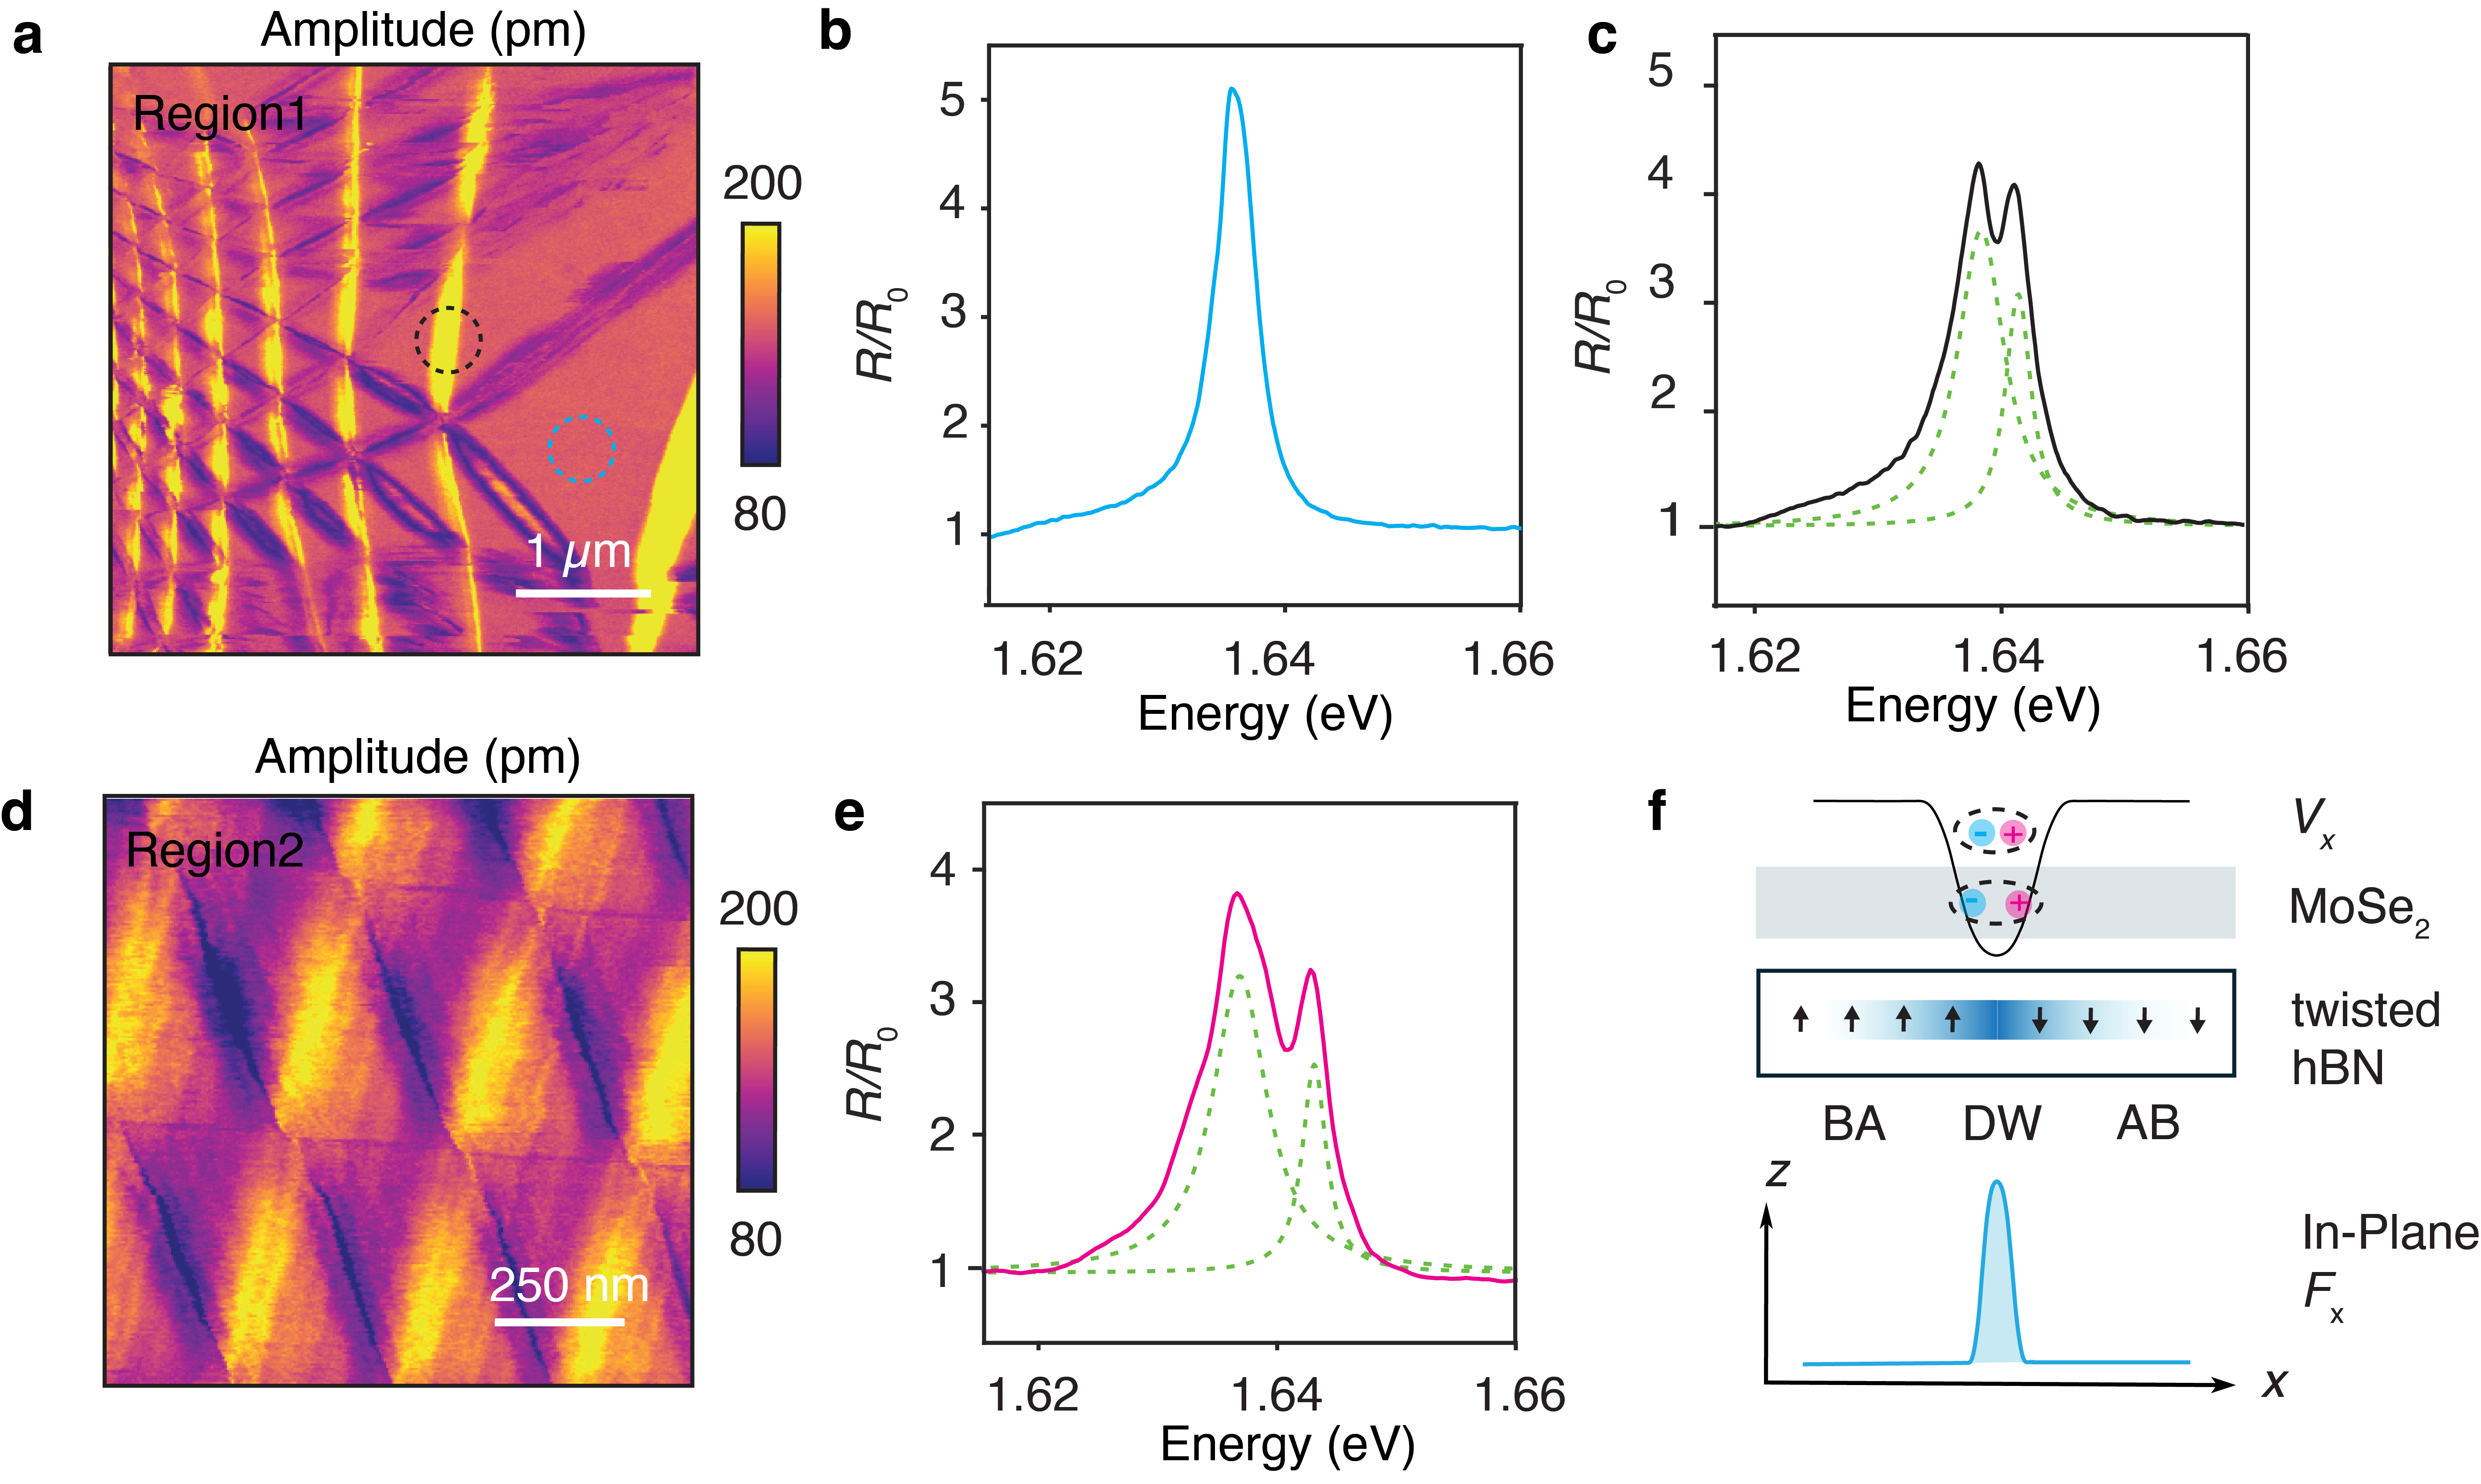
\includegraphics[width=1\textwidth]{Figures/C4/figure2-2.jpg} % 
\end{center}
\caption[caption] {\textbf{Confined intralayer excitons by the in-plane electric field.} \textbf{a,} PFM image of the electrostatic superlattice showing different sizes of triangular domains.\textbf{b,} Normalized reflectance taken at the large domain area indicated as the blue spot in \textbf{a}. \textbf{c,} Normalized reflectance taken at the domain boundary indicated as the black spot in \textbf{a}. Green dashed lines are Lorentzian fit, and the solid line is measured data. \textbf{d,} PFM image of a region with sub-diffraction-limit domains. \textbf{e,} Normalized reflectance spectra taken at the region in \textbf{d}. \textbf{f,} Schematic of the field-induced confinement potential $V_x$ confining intralayer excitons in MoSe$_2$ adjacent to the twisted hBN at the domain boundary.}
\label{fig4.2}
\end{figure}
\end{quote}
\renewcommand{\baselinestretch}{2}
\small\normalsize
% --------------
%%///////////////Figure panel End///////////////////////////

\subsection{1D Confinement nature of excitons}

Excitons confined in 1D potential, such as along moiré domain walls, are expected to exhibit strong anisotropic optical properties\cite{Thureja2022-cv,Bai2020-ih} (Figure~\ref{fig4.3} a). 
Therefore, to test our hypothesis further, we measure how reflectance and PL spectra of the excitons vary as a function of the linear polarization angle. 
First, we study the region with large domains so that only a single domain boundary contributes to the optical signal in the far-field (Figures~\ref{fig4.3} b,c). 
As shown in Figures~\ref{fig4.3} d-f, we observe anisotropic exciton reflection and emission with high degrees of linear polarization. 
By mapping the polarizer direction to the real-space angles on the sample, we find that the exciton polarization directions are parallel to the domain boundaries and remain so across the sample. 
As shown in Figures~\ref{fig4.3} d,e, when the domain wall orientations rotate by $20^\circ$ across two regions, we observe a similar amount of rotation in the linear polarization axis of the excitons. 
In contrast, we did not observe any polarization-dependent behaviors in regions with a single exciton resonance without splitting (Figure~\ref{fig.s2} e). 
Similar exciton splitting and linear polarization behaviors are also observed in more than four different samples with similar structures. 

The observed polarization dependence can be attributed to the 1D confinement at the domain boundary. 
In monolayer TMDs, due to electron-hole exchange interactions, the exciton dispersion splits into longitudinal and transverse branches, which have a coherent superposition of K and -K valley excitons at zero momentum\cite{Yu2014-gi}.
A 1D confinement potential breaks the $C_3$ in-plane rotation symmetry and splits the longitude and transverse branch at the zero momentum, which couples to light in two orthogonal directions \cite{Glazov2015-us,Yu2015-br,Qiu2015-vl} (Figure~\ref{fig.4.3} a).
With sufficiently strong confinement, this x–y polarization energy splitting surpasses the confinement energy, resulting in all confined modes becoming linearly polarized, as observed in our experiments. 
This linear polarization in reflection and emission also strongly suggests that inhomogeneous strain is not the dominant factor here. 
In control experiments observing exciton splitting on non-twisted hBN substrates, the two strain-split exciton resonances have random polarization angle dependence, likely due to variations of the local strain (Fig.~\ref{fig.s3}). 

Furthermore, remarkbly, we find that the 2s exciton state exhibits a larger energy splitting than the 1s state (Figure~\ref{fig.s7}), consistent with its greater polarizability. 
This further supports our conclusion that the splitting is not caused by strain, which would shift the 1s and 2s states by a similar amount.

Consistent with the quantum confinement picture, we find that the lower-energy peak is constantly redshifted relative to the free excitons. 
The higher-energy peak, however, appears near the free exciton energy due to overlapping contributions from both confined and bulk excitons—an effect of our optical probe being much larger than the domain walls.
Additional evidence of exciton confinement comes from power-dependent PL measurements. 
Compared to free 2D excitons, the 1D confined excitons exhibit significantly faster saturation (Figure~\ref{fig.s6}), consistent with the expectation of enhanced exciton–exciton interactions within the confined systems.

Further evidence can also be found in regions where the domain size falls below the diffraction limit. 
In these regions, the exciton reflectance and emission are no longer linearly polarized but still exhibit an anisotropic response. 
Notably, in specific spots, two local maxima of PL emission are observed at polarization angles separated by roughly sixty degrees (Figure.~\ref{fig.s2} d). 
These phenomena can be understood from the non-perfect triangle shapes of domain boundaries measured from PFM, where one particular domain wall direction would contribute more to the measured optical signal than the other directions.

%///////////////////////Figure Panel/////////////////////////

%Fig.4--------------
\renewcommand{\baselinestretch}{1}
\small\normalsize
\begin{quote}
\begin{figure}
\begin{center}
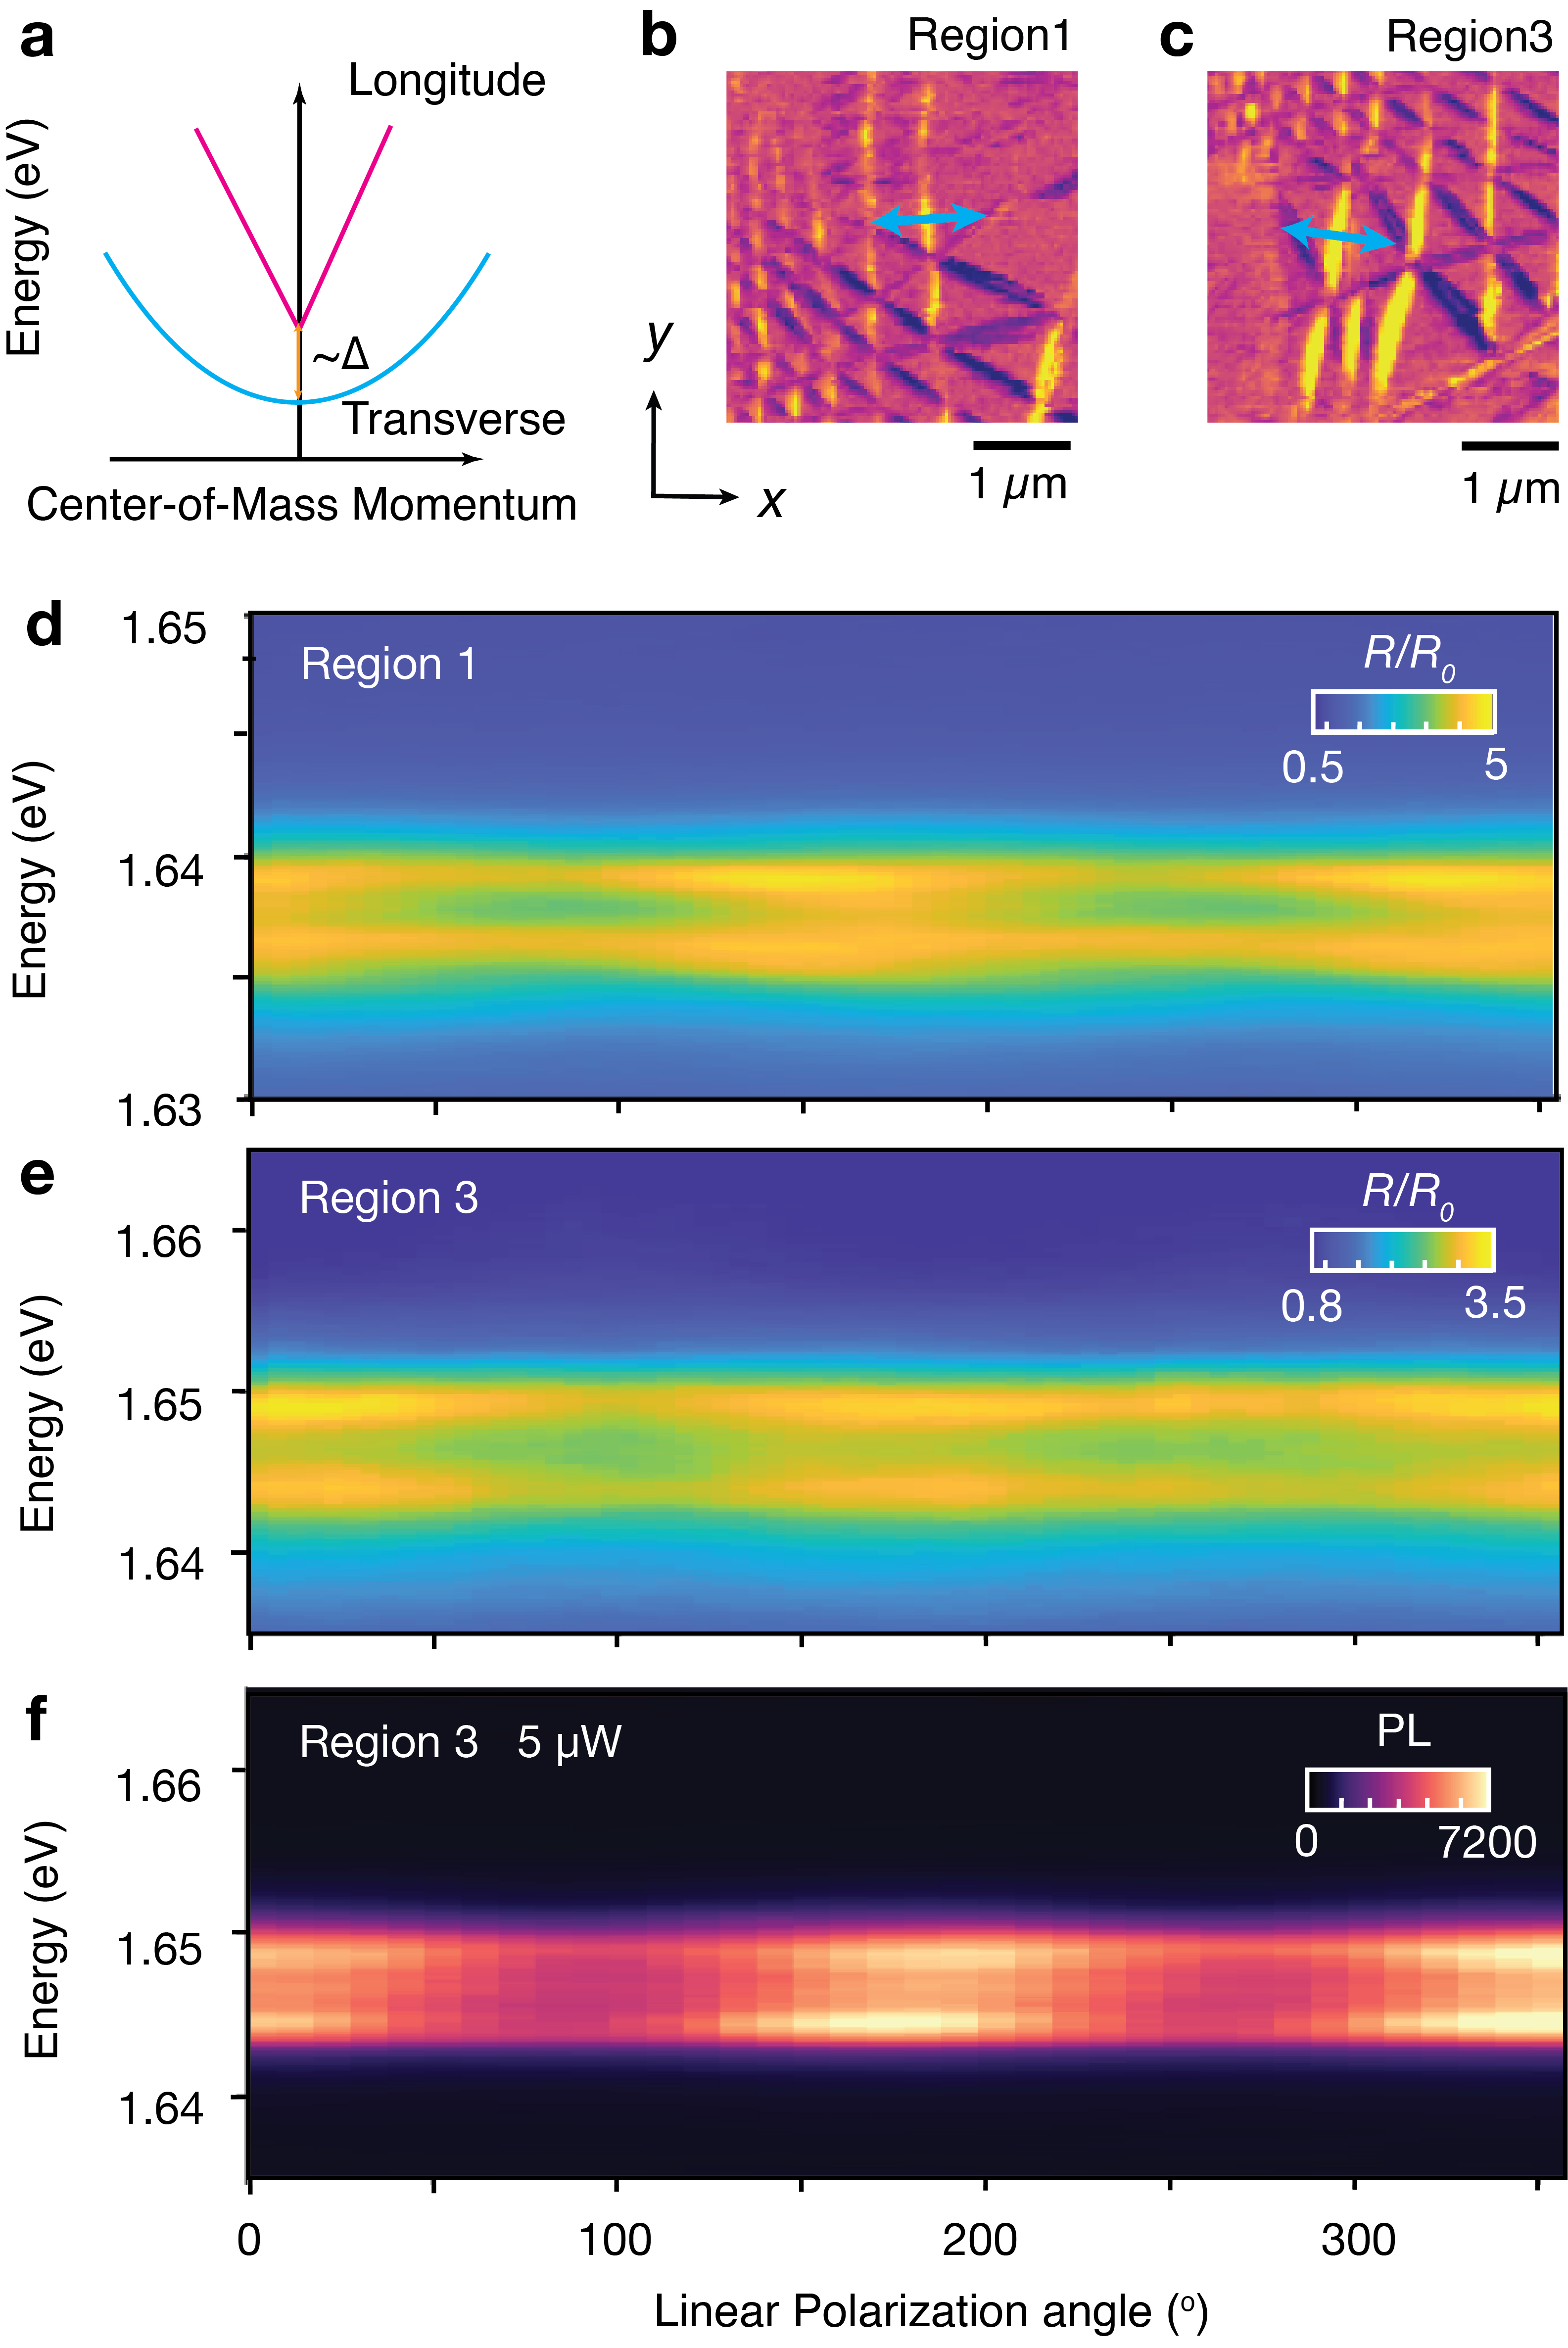
\includegraphics[width=0.7\textwidth]{Figures/C4/figure3-7.jpg} % 
\end{center}
\caption[caption] {\textbf{1D confinement at the domain boundary.} \textbf{a,} Schematic of the confined exciton dispersion. Under spatial localization, the exciton longitude and transverse branch become split with a magnitude of $\sim\Delta$ at zero center-of-mass momentum.\textbf{b,c,} PFM map of \textbf{b,} regions 1 and \textbf{c,} regions 3. \textbf{d,e,} Normalized reflectance as a function of the excitation linear polarization angle in regions 1 and 3 as indicated by the blue arrow in \textbf{b} and \textbf{c}, respectively. \textbf{f,} PL emission as a function of linear polarization with $5\,\mu\mathrm{W}$ excitation power from $635\,\mathrm{nm}$ CW laser. The spot is the same one taken in \textbf{e}.}
\label{fig4.3}
\end{figure}
\end{quote}
\renewcommand{\baselinestretch}{2}
\small\normalsize
% --------------

%Fig.5--------------
\renewcommand{\baselinestretch}{1}
\small\normalsize
\begin{quote}
\begin{figure}
\begin{center}
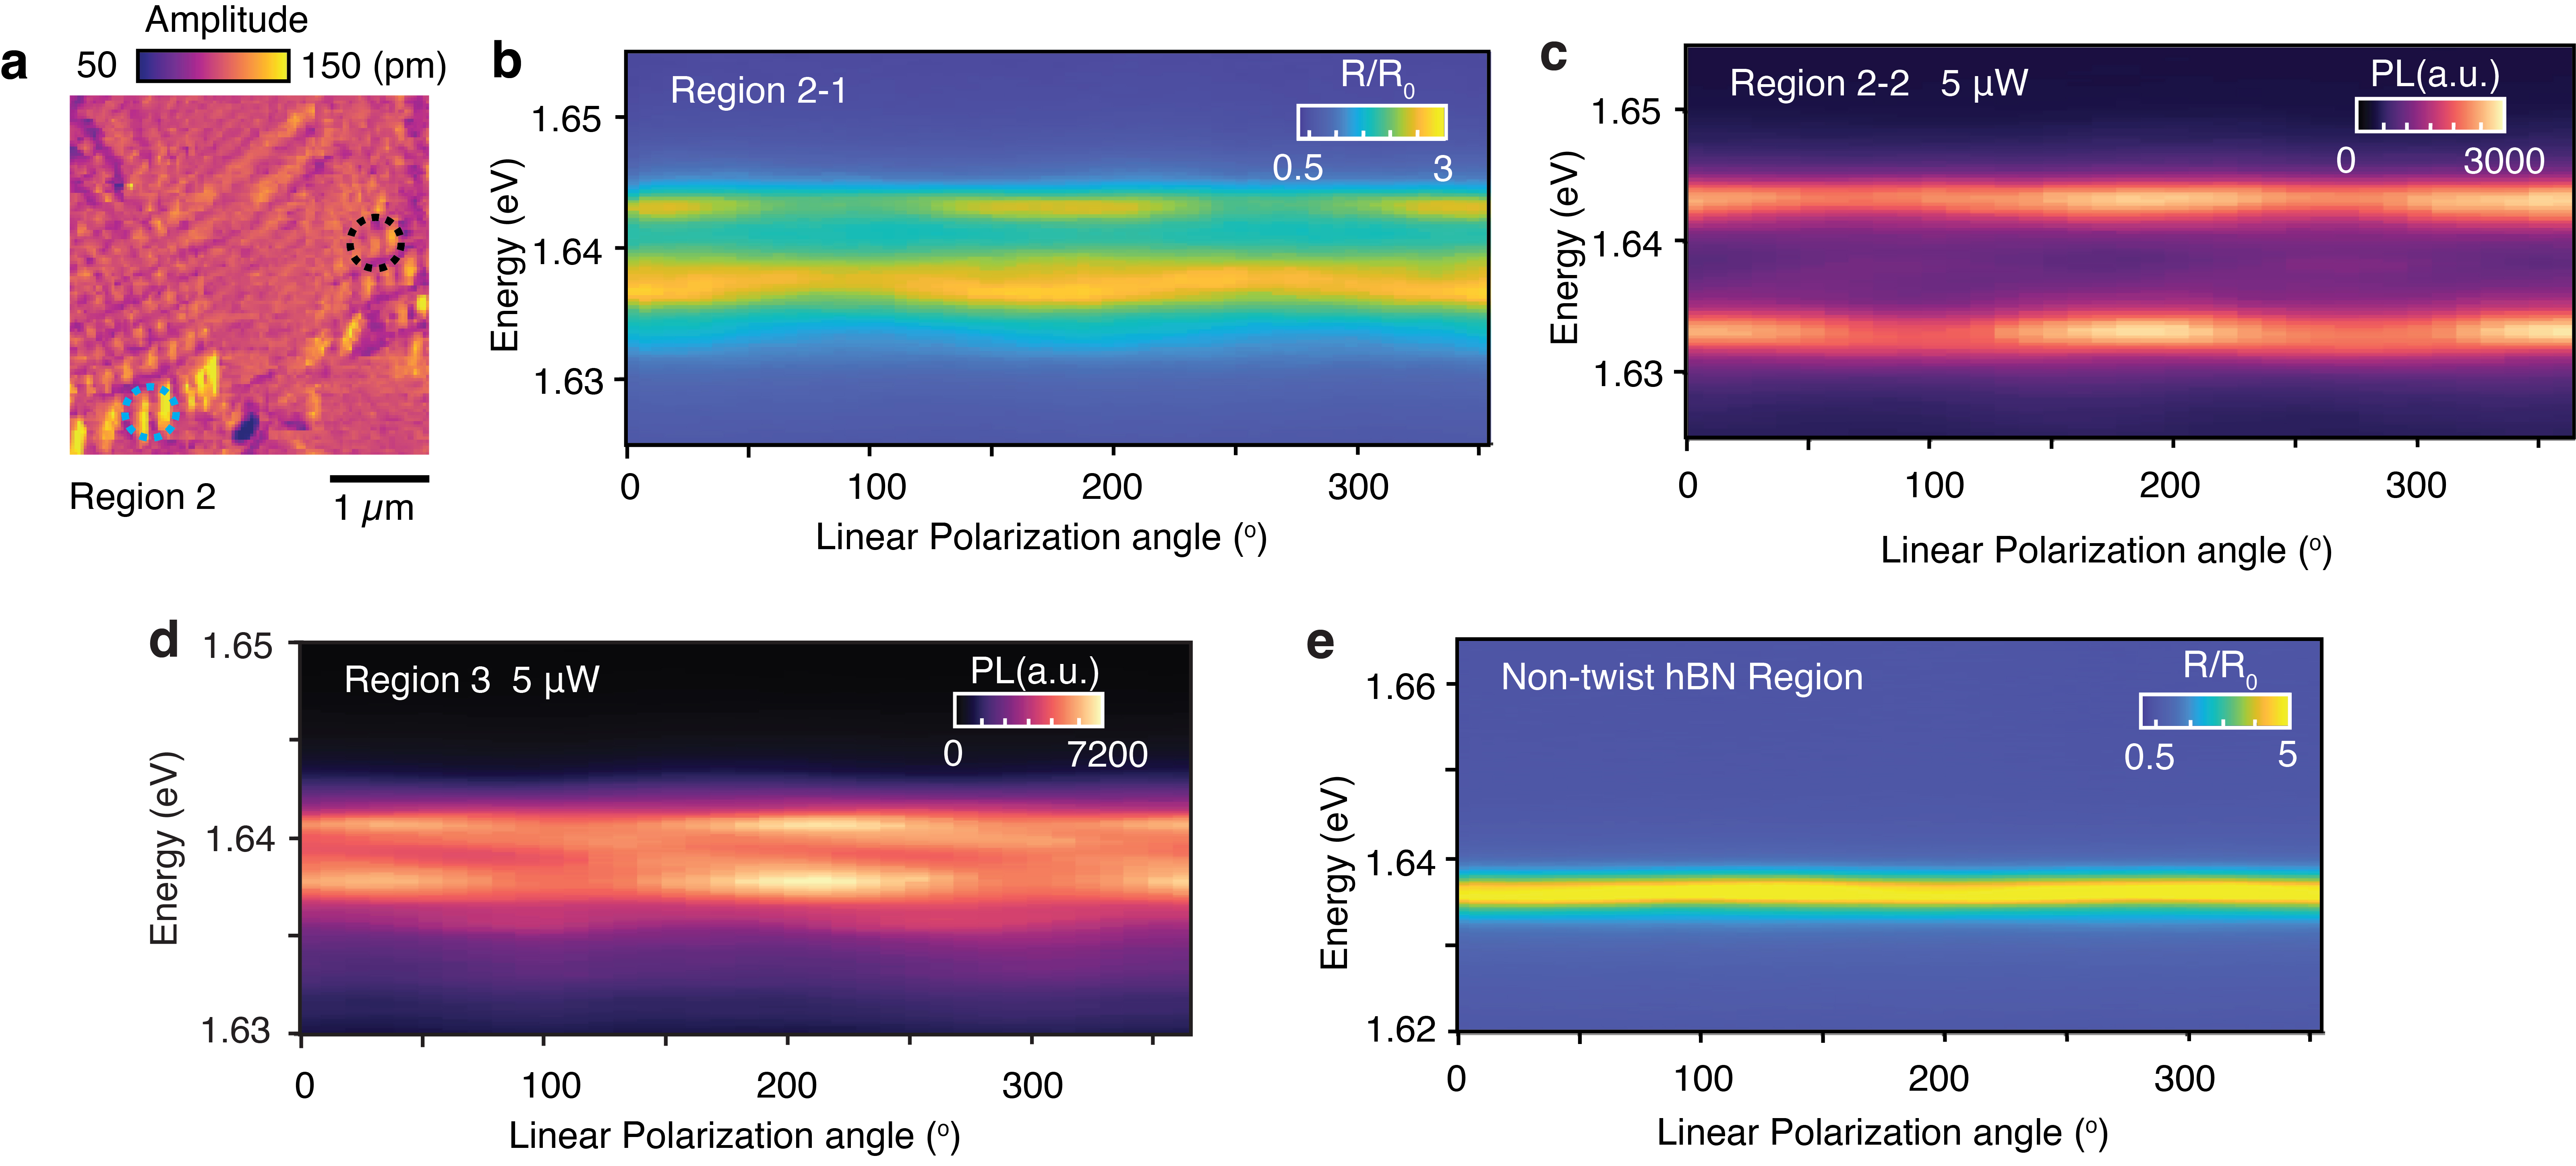
\includegraphics[width=1\textwidth]{Figures/C4/figure-S2.jpg} % 
\end{center}
\caption[caption] {\textbf{Polarization dependence of excitons in regions with sub-diffraction domains.} \textbf{a,} PFM amplitude map of region 2. The blue and black dashed circles correspond to the detection spot in \textbf{b} and \textbf{c}, respectively. 
\textbf{b,} Linear polarization dependence of the exciton reflection in region 2-1. \textbf{c,} Linear polarization dependence of PL in regions 2-2, which has a small domain size below the diffraction limit (smaller than 200 nm). The splitting energy of the two resonances is around 10 meV. \textbf{d,} Linear polarization PL emission for the similar spot in Fig.~\ref{fig4.3} b (region 2). As the laser spot detects two domains simultaneously, there are two maxima in the PL polarization angle, which are separated by a nearly $60^\circ$. This can be understood from the non-perfect triangle shapes of domain boundaries measured from PFM, where one particular domain wall direction would contribute more to the measured optical signal than the other directions. \textbf{e,} Linear polarization dependence of the reflectance taken at the non-twist hBN region. No obvious polarization dependence is observed. }
\label{fig.s2}
\end{figure}
\end{quote}
\renewcommand{\baselinestretch}{2}
\small\normalsize
% --------------

%Fig.6--------------
\renewcommand{\baselinestretch}{1}
\small\normalsize
\begin{quote}
\begin{figure}
\begin{center}
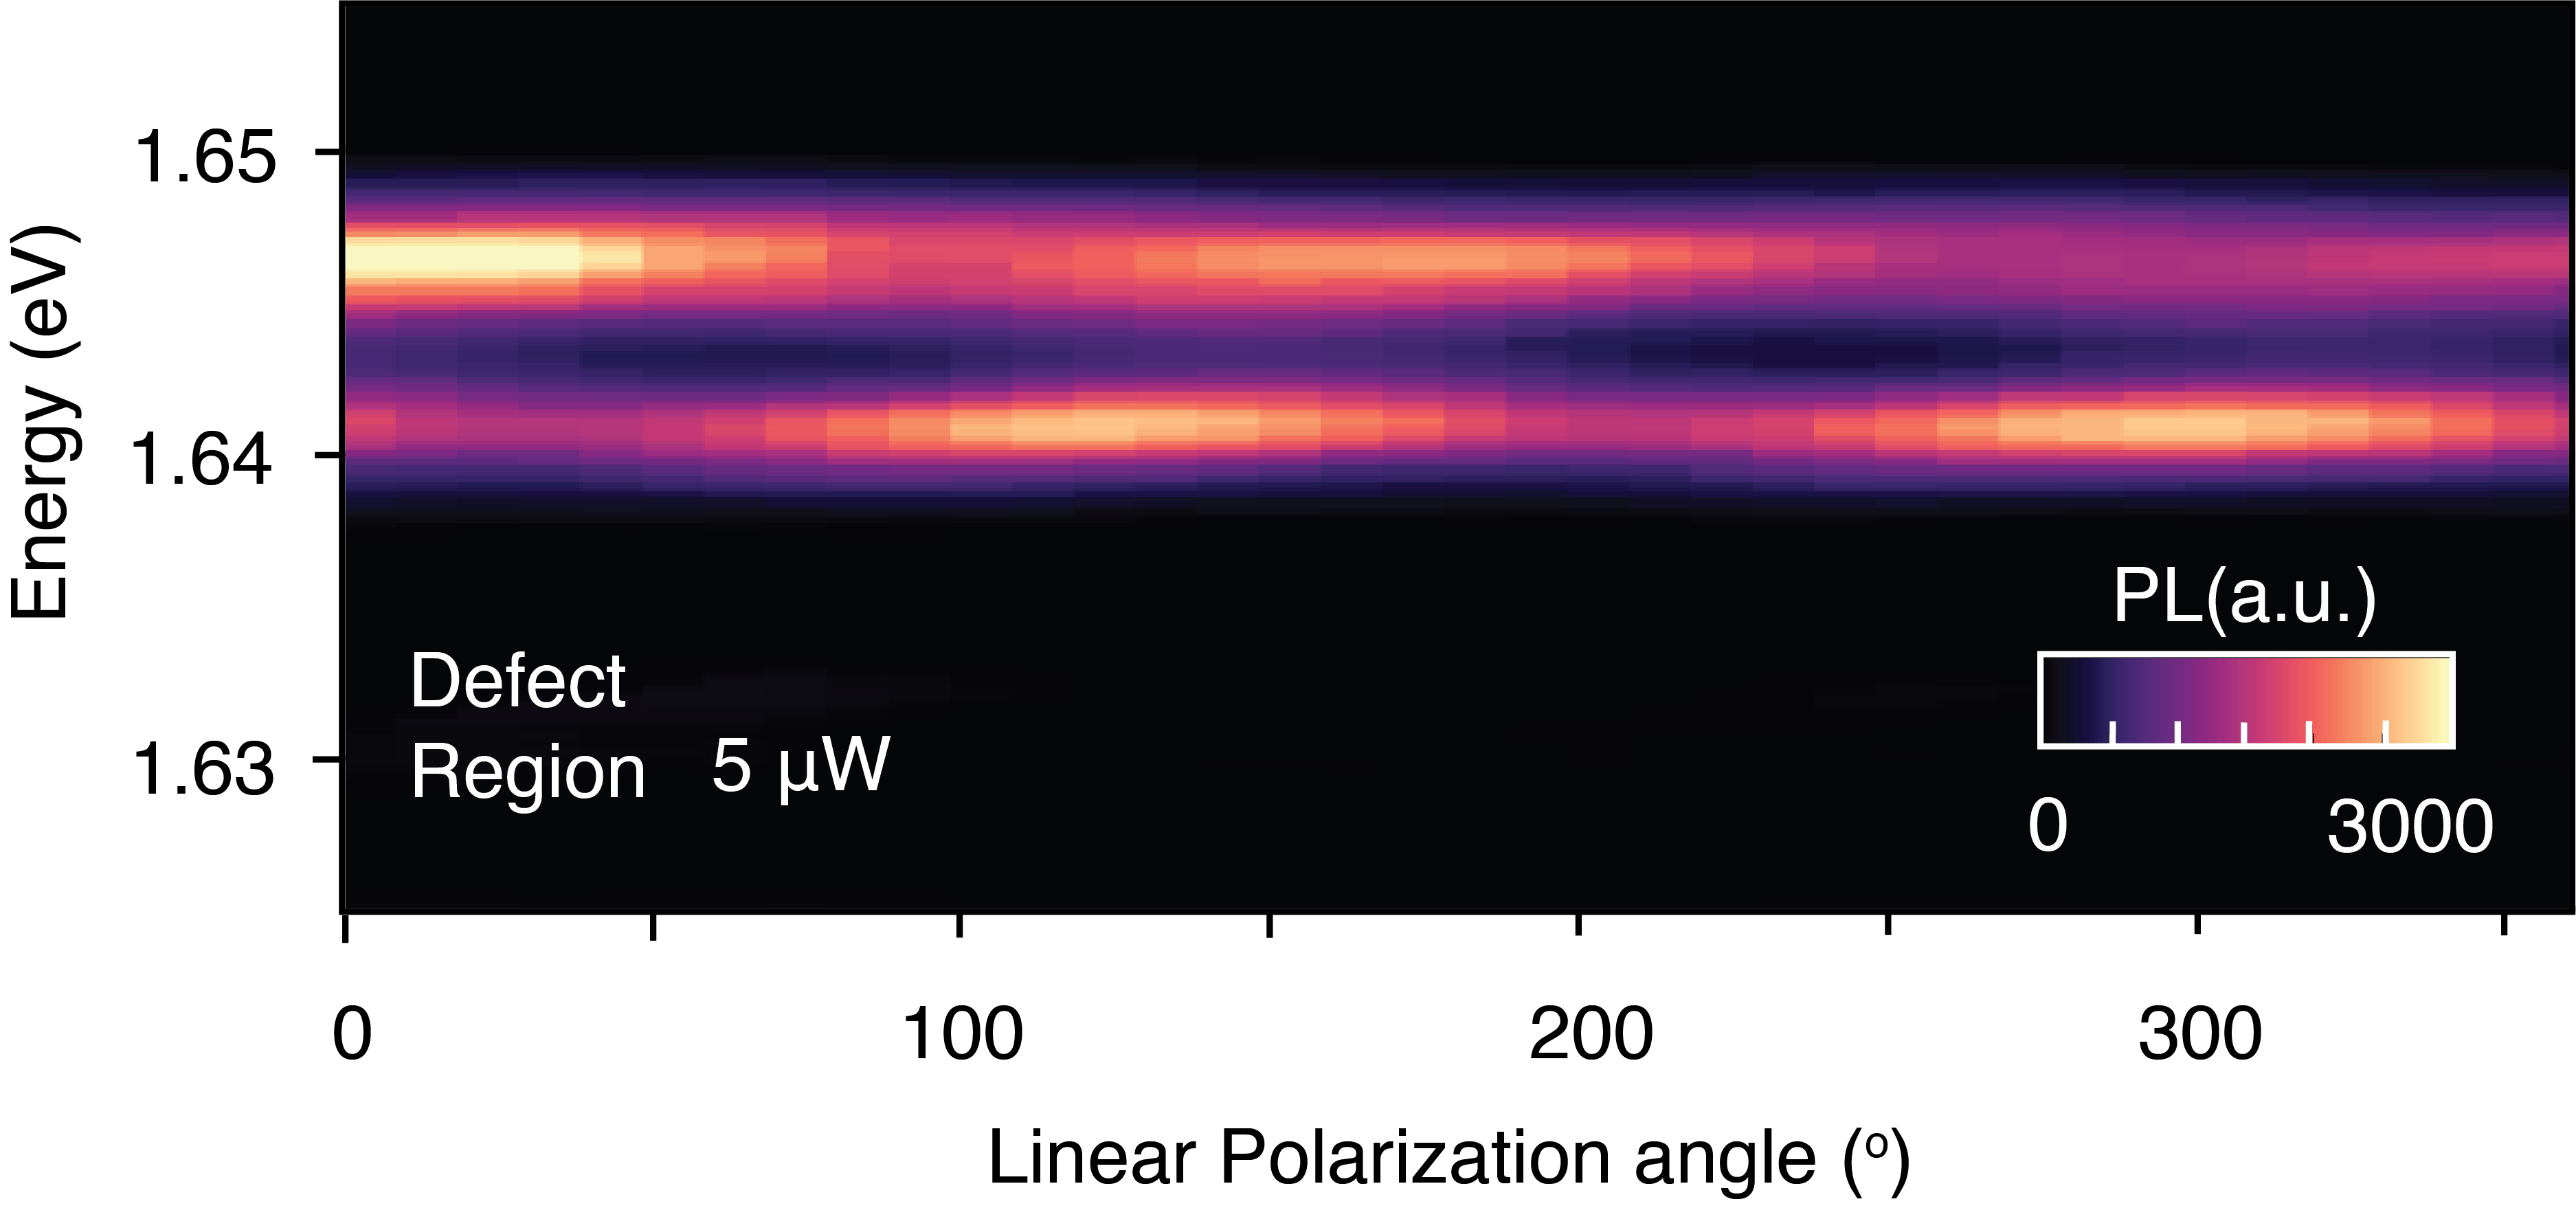
\includegraphics[width=0.7\textwidth]{Figures/C4/figure-S3.jpg} % 
\end{center}
\caption[caption] {\textbf{Polarization dependence of energy-split excitons caused by strain} In regions where local strain splits the exciton peaks, the two exciton peaks do not have the same linear polarization.}
\label{fig.s3}
\end{figure}
\end{quote}
\renewcommand{\baselinestretch}{2}
\small\normalsize
% --------------

%Fig.7--------------
\renewcommand{\baselinestretch}{1}
\small\normalsize
\begin{quote}
\begin{figure}
\begin{center}
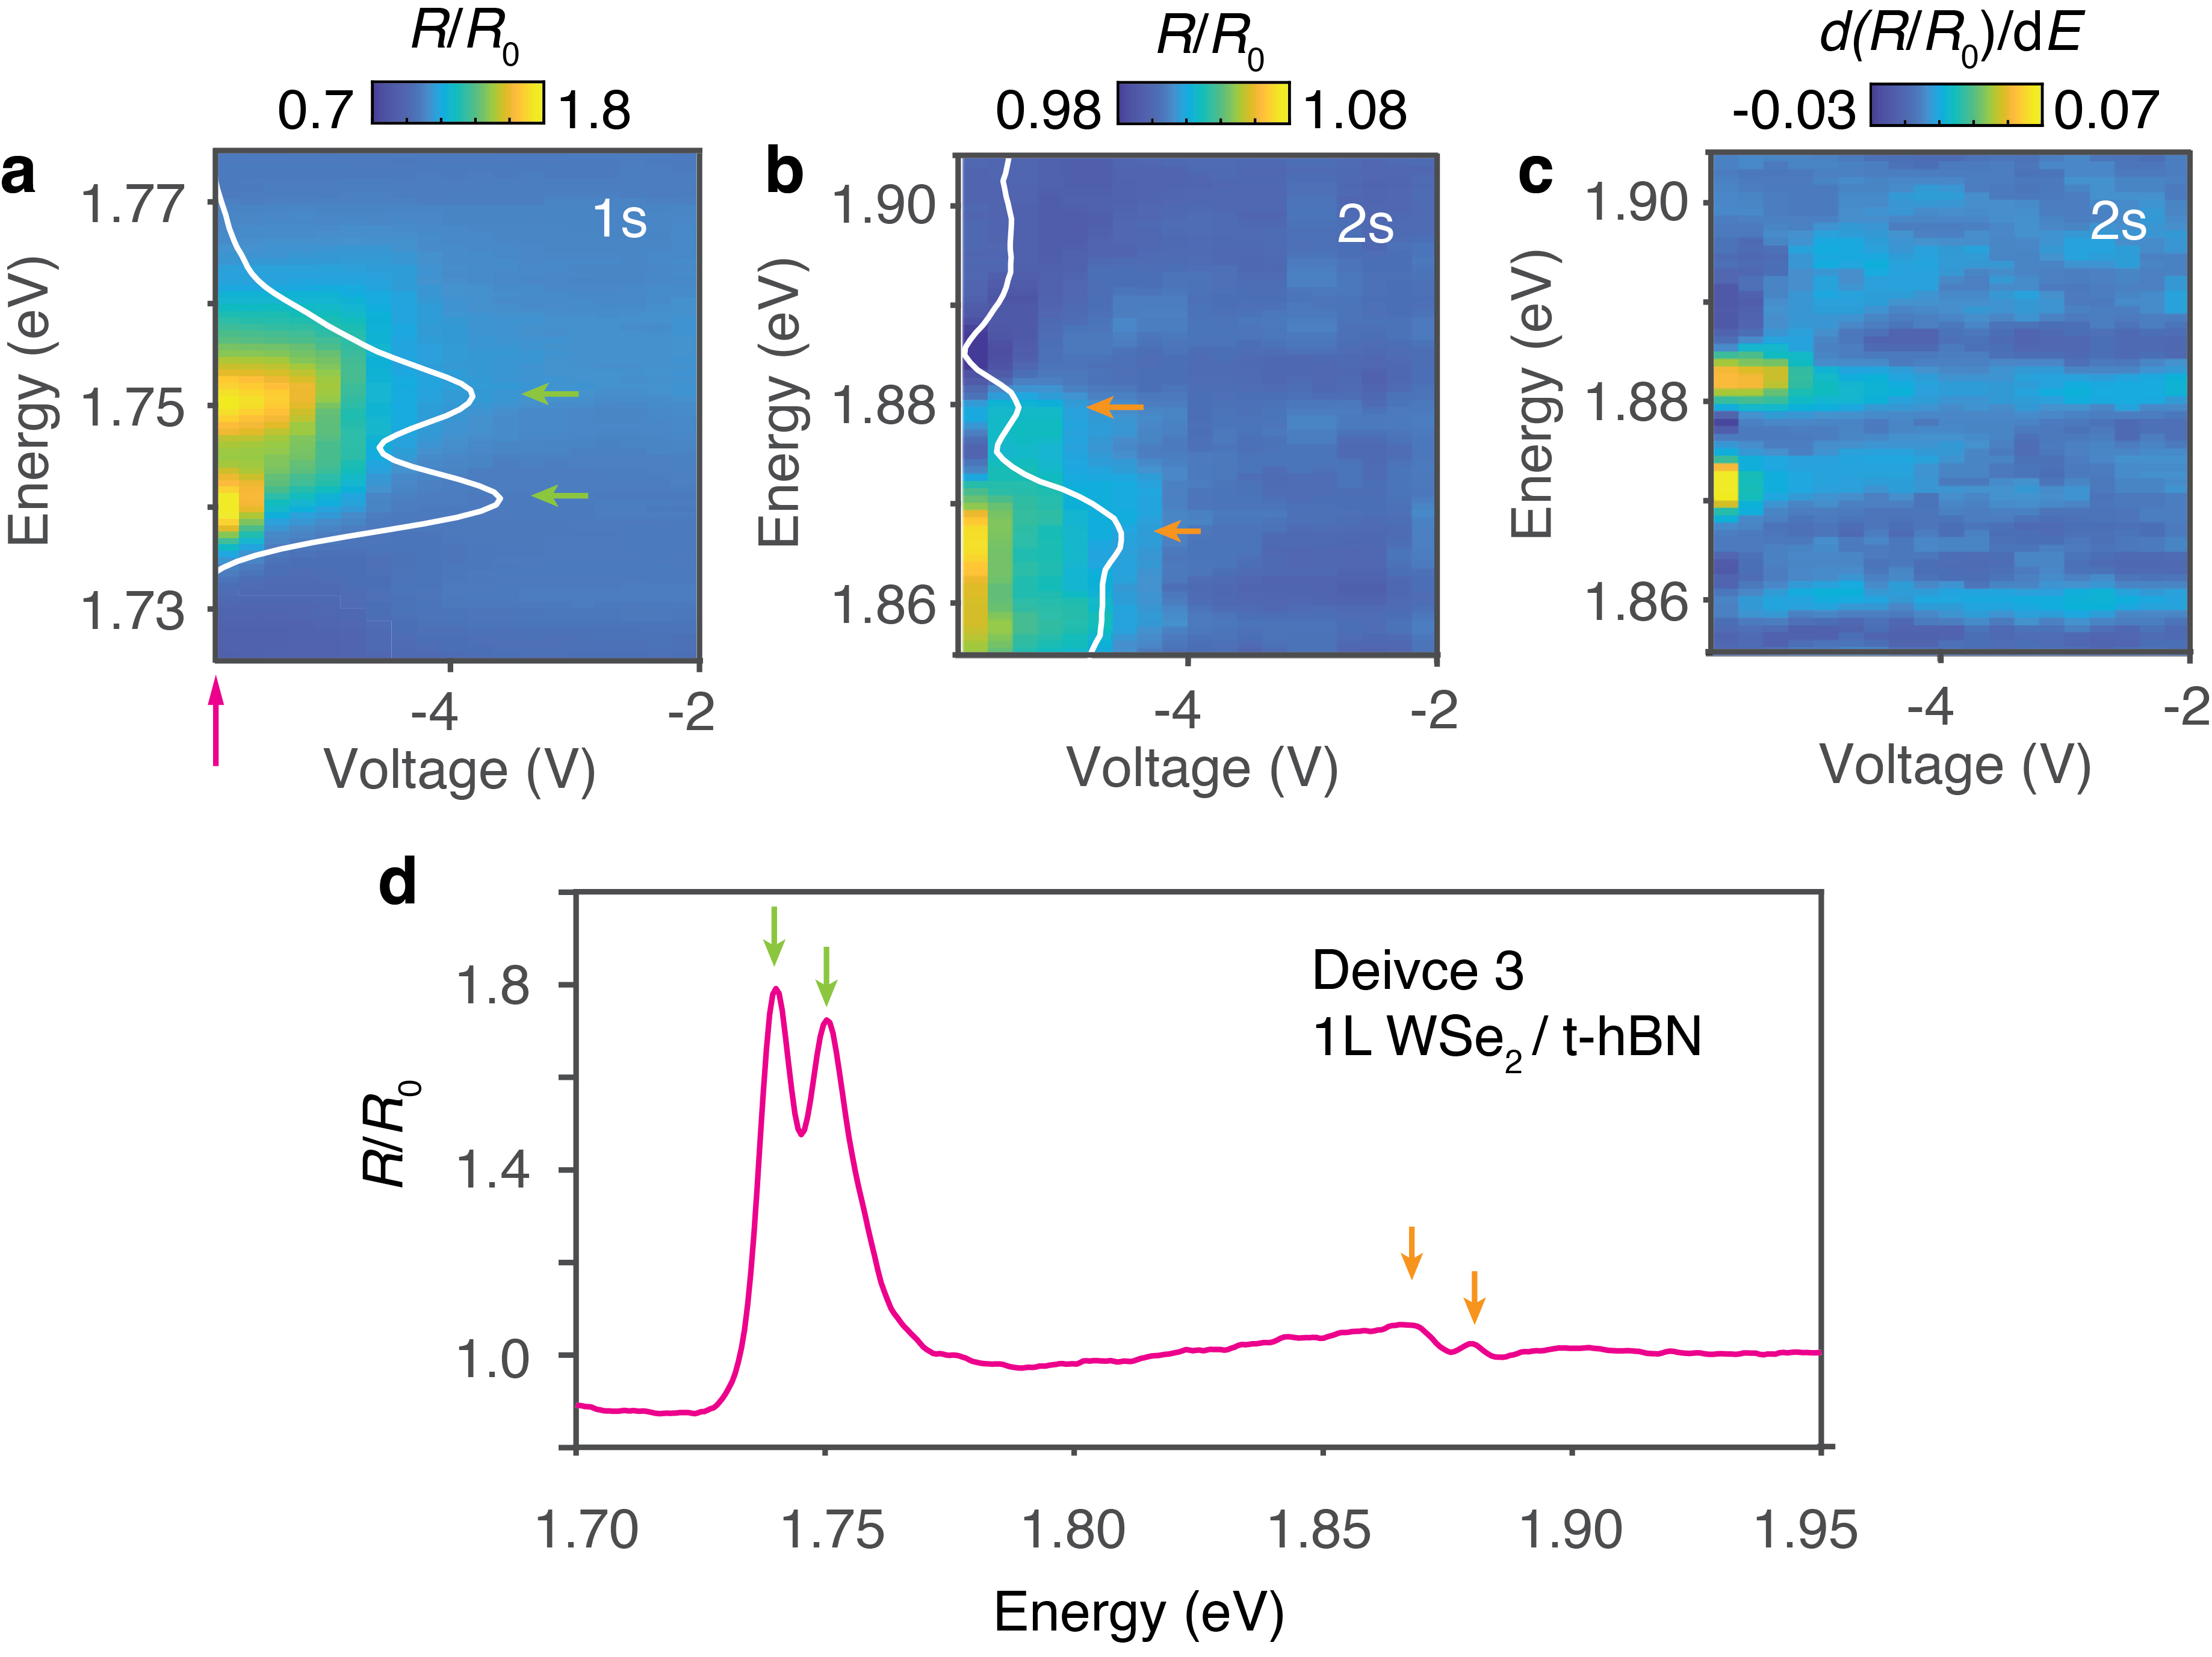
\includegraphics[width=0.8\textwidth]{Figures/C4/figure-S7.jpg} % 
\end{center}
\caption[Rydberg exciton] {\textbf{Quantum confinement of 2S exciton in 1L $WSe_2$ / twisted hBN.} \textbf{a,} 1s exciton and \textbf{b,} 2s exciton splitting shown in normalized reflectance. \textbf{c,} Normalized reflectance spectrum at charge neutral point. The energy splitting is $\sim$ 10 meV for 1s exciton and $\sim$ 13 meV for 2s exciton. For monolayer $WSe_2$ on the same twisted hBN interface, a larger energy splitting than that of MoSe$_2$ is expected due to a larger polarizability of $\alpha \sim 10.2~\text{eV}\,\text{nm}^2/\text{V}^2$ in $WSe_2$ for 1s exciton. The 2s exciton owns even larger splitting due to its large Bohr radius and thus larger polarizability.}
\label{fig.s7}
\end{figure}
\end{quote}
\renewcommand{\baselinestretch}{2}
\small\normalsize
% --------------


%Fig.8--------------
\renewcommand{\baselinestretch}{1}
\small\normalsize
\begin{quote}
\begin{figure}
\begin{center}
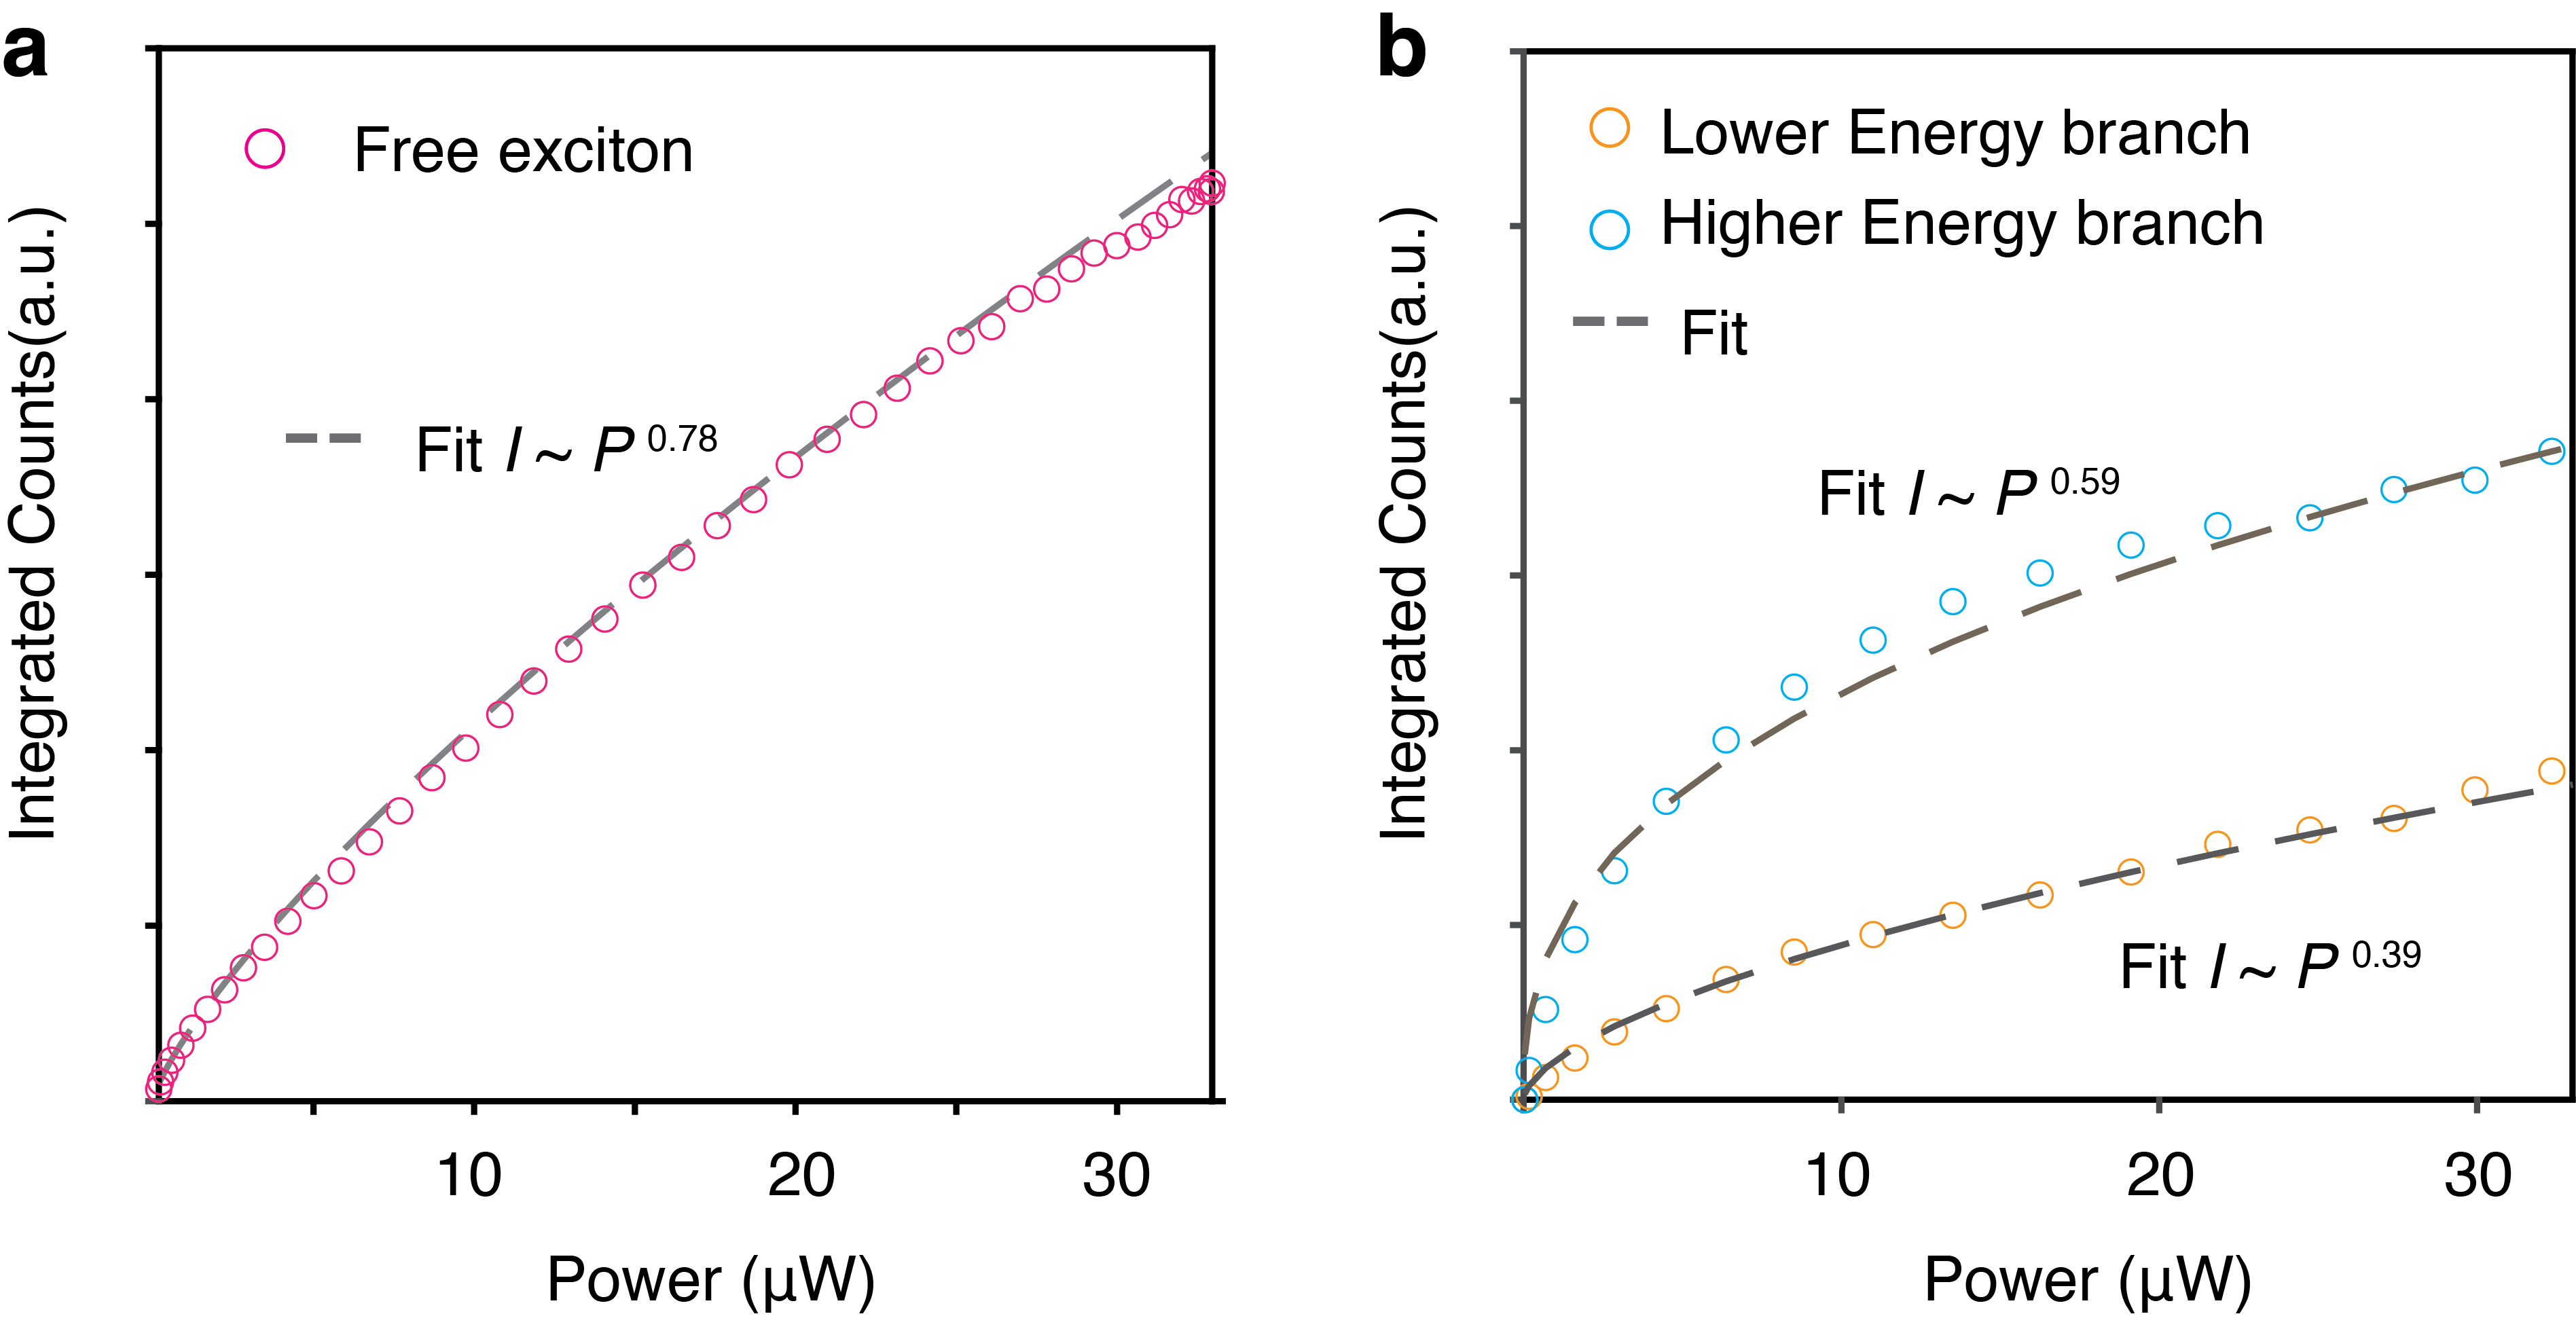
\includegraphics[width=0.7\textwidth]{Figures/C4/figure-S6.jpg} % 
\end{center}
\caption[power dependent] {\textbf{Excitation power–dependent PL intensities of free and 1D-confined excitons.} With increasing excitation power, \textbf{a,} the integrated PL intensity of free 2D excitons rises almost linearly, whereas \textbf{b,} the 1D-confined excitons exhibit sublinear saturation. Notably, the lowest-energy branch saturates significantly faster than the higher-energy branch.}
\label{fig.s6}
\end{figure}
\end{quote}
\renewcommand{\baselinestretch}{2}
\small\normalsize
% --------------
%///////////////////////Figure Panel End/////////////////////////

\subsection{Anisotropic Polarization of polarons and temperature-dependent}

Such quantum confinement also applies to charged excitons near DBs. 
In another MoSe$_2$ device, D2, we also observe a splitting in both the repulsive and the attractive polarons as we adjust the doping levels via gating (Figure~\ref{fig.s4}).
The reflectance of the neutral exciton, repulsive polaron, and attractive polaron all exhibit linear polarization parallel to the domain wall directions, indicating that 1D confinement can also occur for the Fermi polarons (Figures~\ref{fig.4-10} a-c).
Intriguingly, as doping density increases, the split between the repulsive polarons tends to decrease, whereas that between the attractive polarons slightly increases (Figure~\ref{fig.s4} b).
A quantitative understanding of the confinement of Fermi polarons requires further theoretical studies, for instance, on the polarizability of attractive vs. repulsive polarons \cite{Cavalcante2018-er}. 
Nevertheless, such behaviors stand in stark contrast to strain-induced energy splitting, which is expected to be independent of doping. 

To further demonstrate the robustness of this confinement, we measure the polarization-resolved reflectance of the neutral excitons at different temperatures. 
The anisotropic excitonic response persists but becomes weaker with increasing temperature. 
At temperatures around 80 K, where the thermal energy becomes comparable to the confinement potential, the two split exciton peaks merge into a single free exciton peak. 
The reflection and emission from excitons also become isotropic in the 2D plane above this temperature. 
We note that the disappearance of the splitting is not simply due to the linewidth change because the total linewidth does not change dramatically with increasing temperature up to 100 K (Figure~\ref{fig.s5}). 

%////////////////////////////Figure Panel//////////////////
%Fig.9(s4)--------------
\renewcommand{\baselinestretch}{1}
\small\normalsize
\begin{quote}
\begin{figure}
\begin{center}
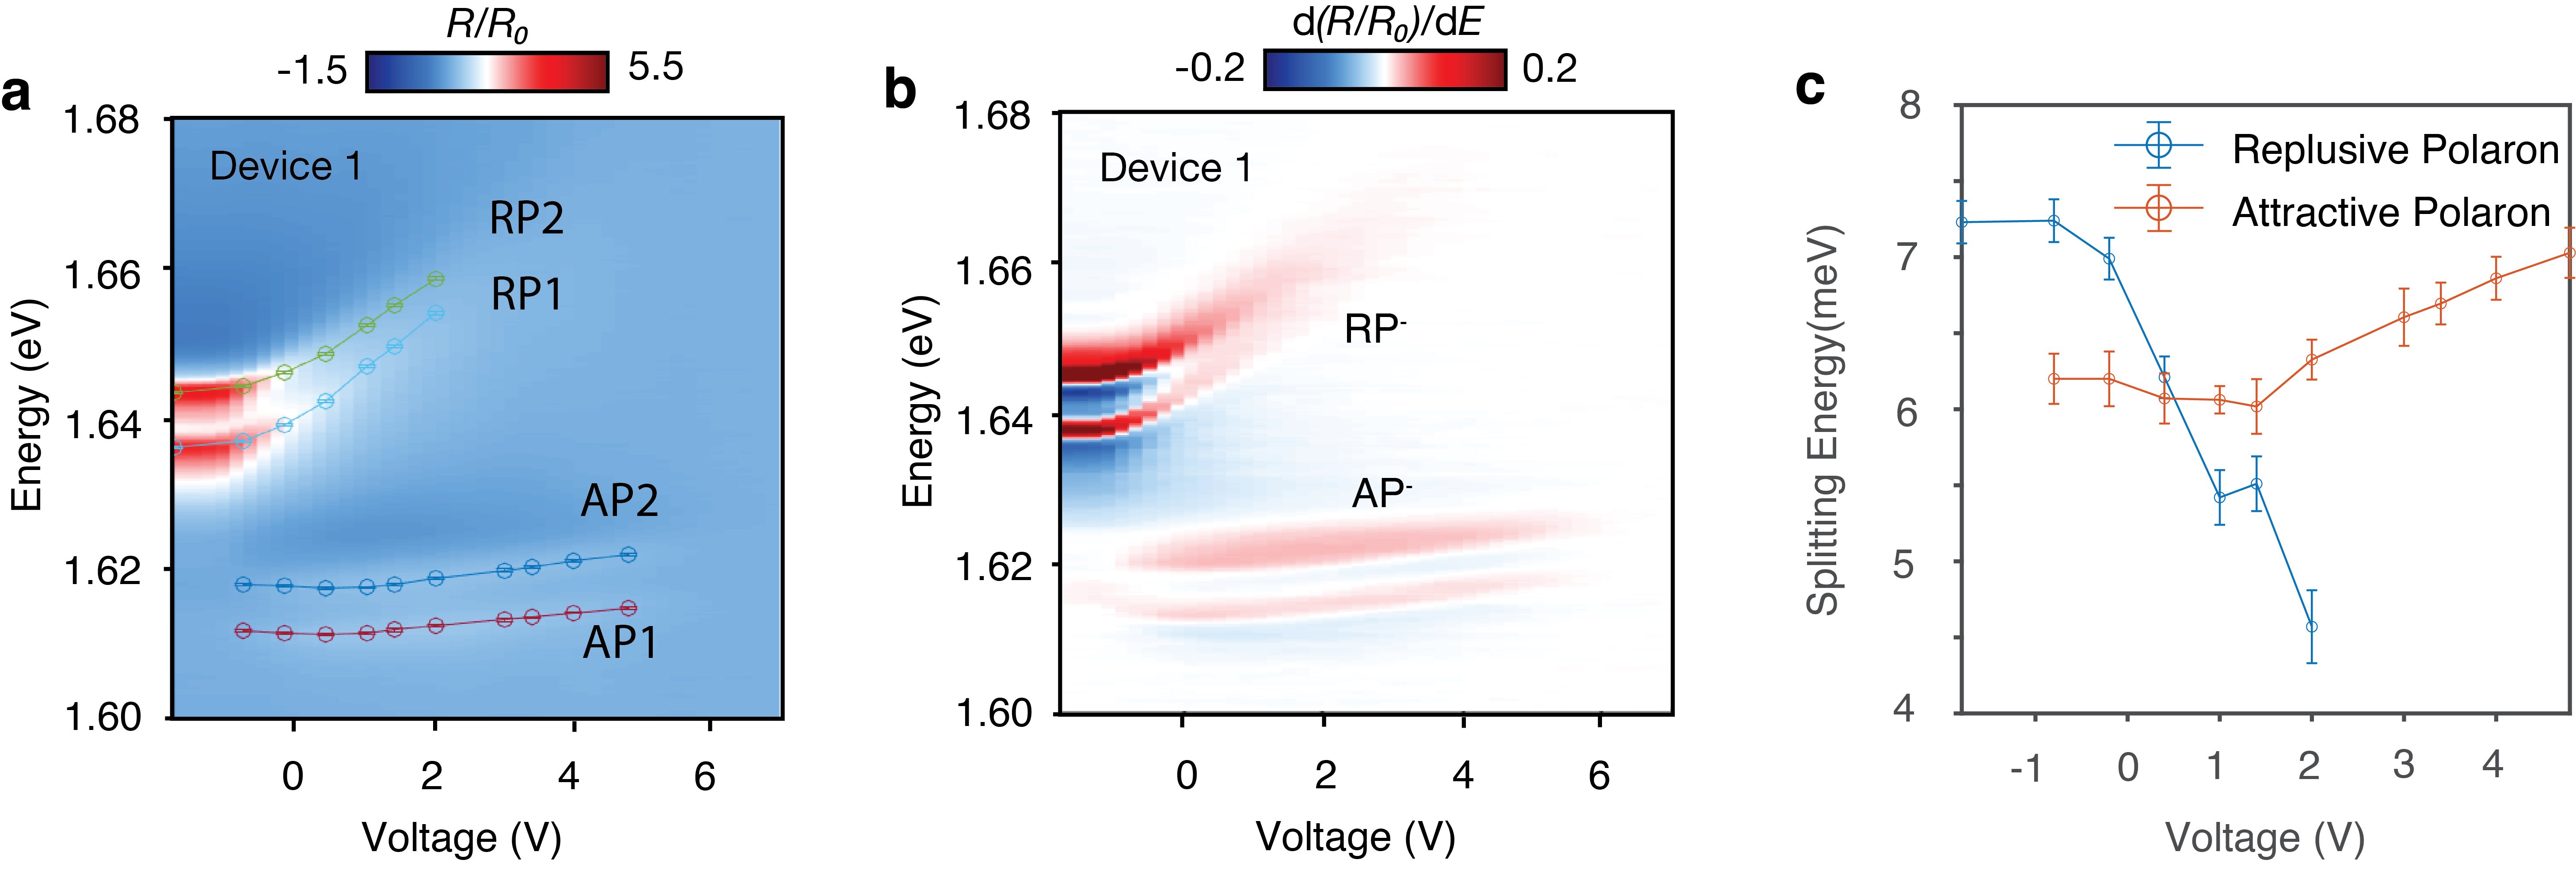
\includegraphics[width=1\textwidth]{Figures/C4/figure-S4.jpg} % 
\end{center}
\caption[gate polarons] {\textbf{Confinement of repulsive and attractive polarons.} Doping dependence of \textbf{a,} normalized reflectance, and \textbf{b,} its derivative with respect to energy. 
\textbf{c,} The energy splitting of the repulsive and attractive polarons exhibit different dependence on the doping level. The error bars represents the uncertainty in determining the peak position by Gaussian fit.}
\label{fig.s4}
\end{figure}
\end{quote}
\renewcommand{\baselinestretch}{2}
\small\normalsize
% 

%Fig.10(4)--------------
\renewcommand{\baselinestretch}{1}
\small\normalsize
\begin{quote}
\begin{figure}
\begin{center}
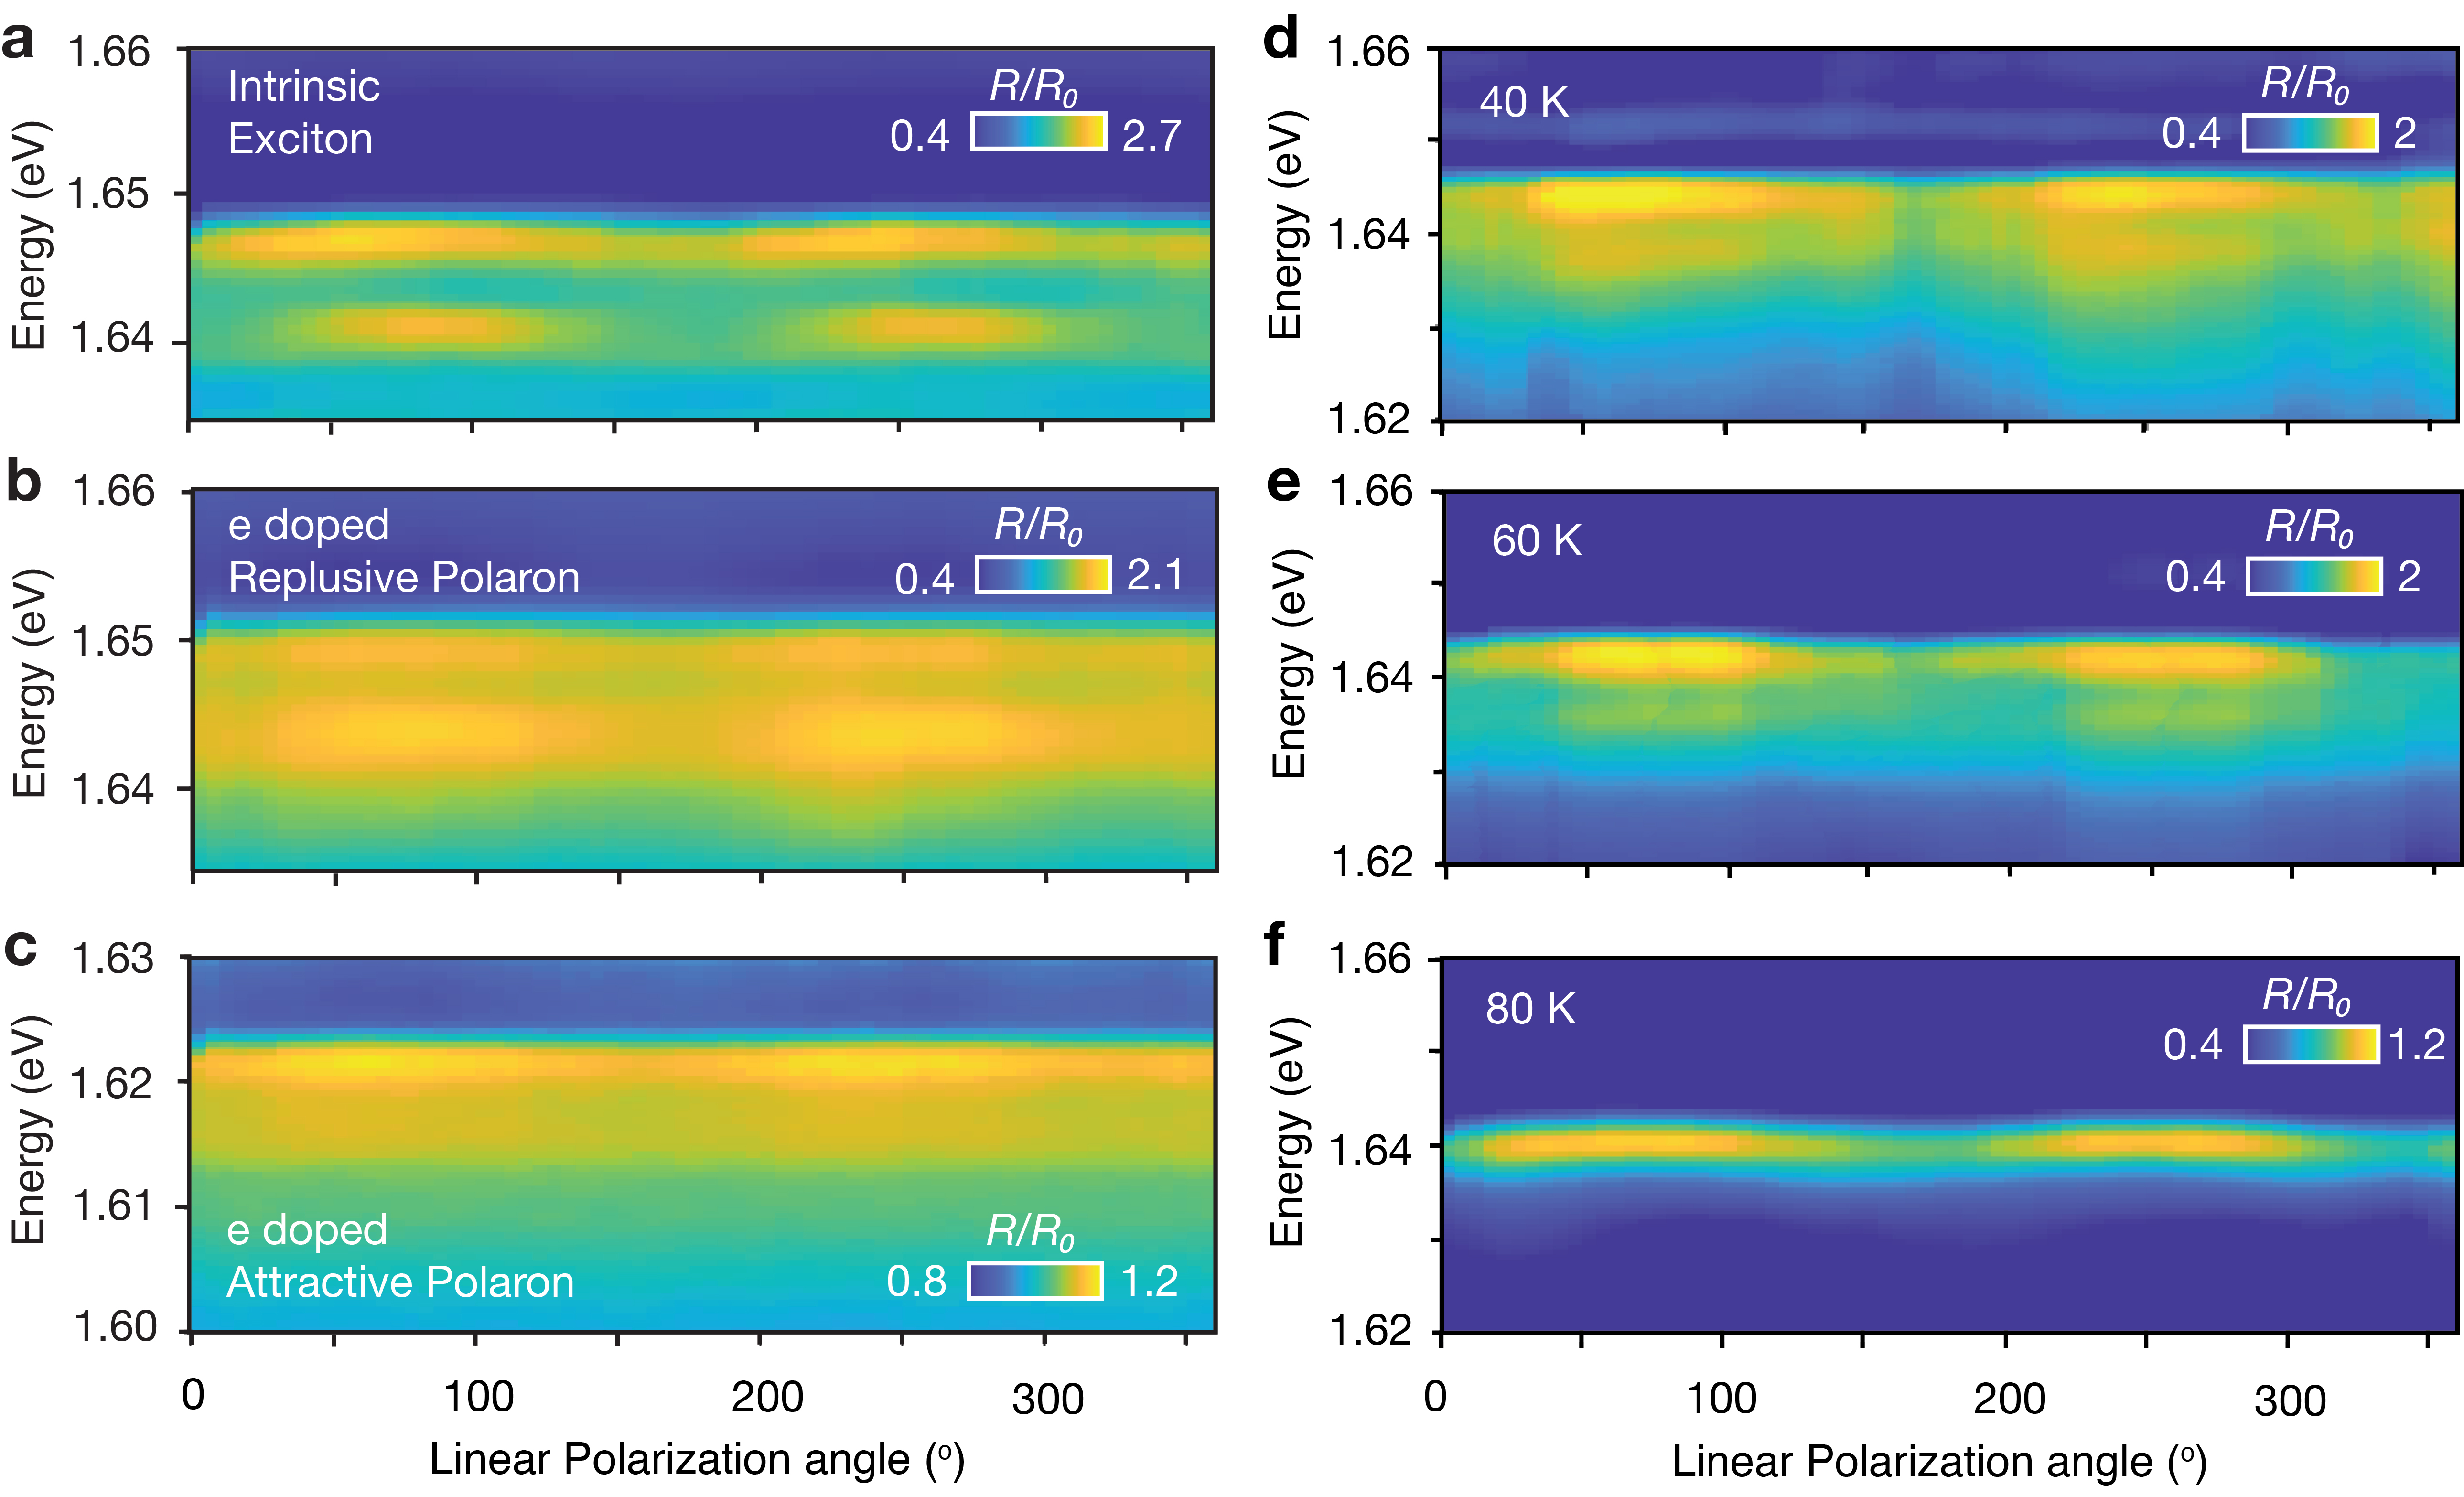
\includegraphics[width=0.9\textwidth]{Figures/C4/figure4-9.jpg} % 
\end{center}
\caption[gate polarons polarization] {\textbf{Anisotropic optical response of Fermi polarons and their temperature dependence.} \textbf{a-c,} Linear polarization dependent reflectance of a, neutral exciton (at gate voltage \textit{V} =-2.5 V), \textbf{b,} repulsive polaron, and \textbf{c,} attractive polaron (at gate voltage \textit{V} =0.5 V) at electron-doped in MoSe$_2$ in device \textbf{D2} at 5 K. \textbf{d-f,} Linear polarization dependent reflectance of neutral exciton at different temperatures.}
\label{fig.4-10}
\end{figure}
\end{quote}
\renewcommand{\baselinestretch}{2}
\small\normalsize
% 

%Fig.11(s5)--------------
\renewcommand{\baselinestretch}{1}
\small\normalsize
\begin{quote}
\begin{figure}
\begin{center}
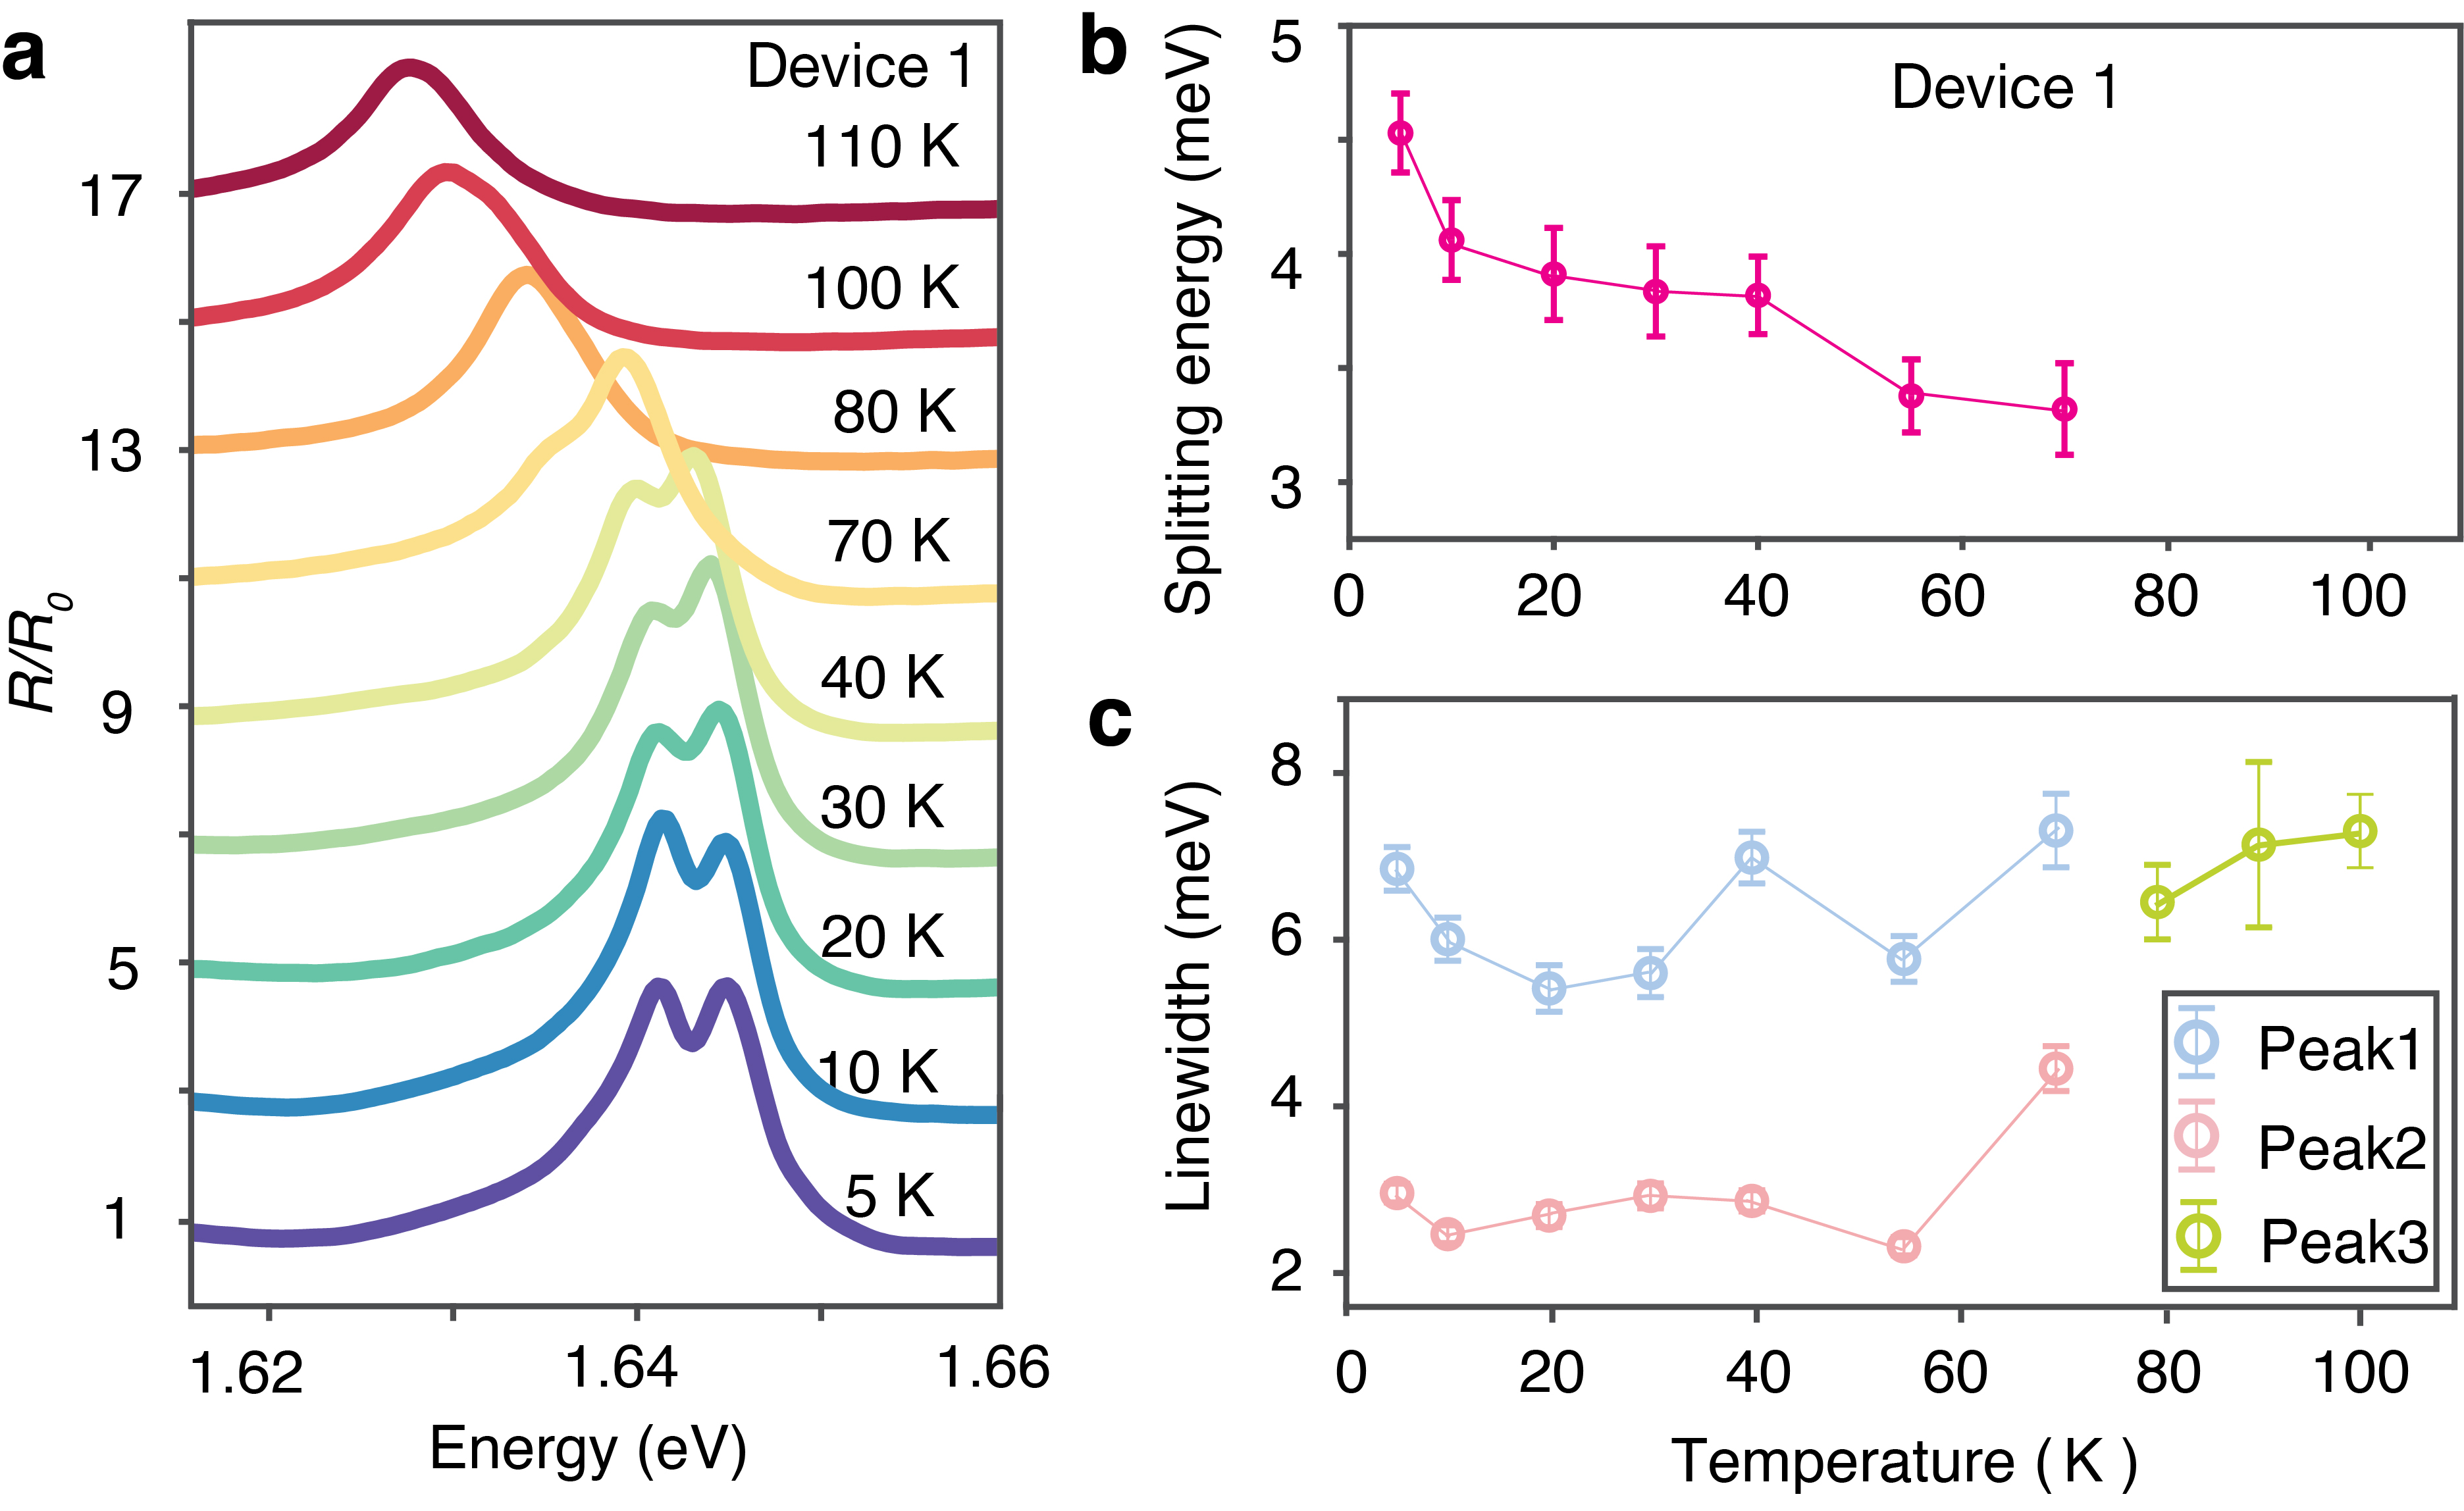
\includegraphics[width=0.9\textwidth]{Figures/C4/figure-S5.jpg} % 
\end{center}
\caption[Temperature dependent QC] {\textbf{Temperature-dependent quantum confinement.} \textbf{a-c,} \textbf{a,} Normalized reflectance of the intralayer excitons at different temperatures. With increasing temperature, each spectrum is shifted by a constant. \textbf{b,} The splitting energy decreases with increasing temperature and eventually vanishes near 80 K. \textbf{c,} The extracted linewidth as a function of temperature. Below 100 K, the linewidth does not change significantly, suggesting that the observed reduction in the splitting energy is not simply due to the linewidth change. The error bars represent the uncertainty associated with the fitted parameters of a Lorentzian model.}
\label{fig.s5}
\end{figure}
\end{quote}
\renewcommand{\baselinestretch}{2}
\small\normalsize
%////////////////////////////Figure Panel End//////////////////

\section{Discussions}

Finally, we quantify the strength and spatial extent of the quantum confinement potential. 
The potential depth induced by the in-plane electric field is given by Eq.~\ref{eq:stark}, 
where $\alpha\sim 6.5~\text{eV}\,\text{nm}^2/\text{V}^2$ for intralayer excitons in monolayer MoSe$_2$\cite{Thureja2022-yc,Cavalcante2018-er}. 
By modelling the electrostatic field generated by twisted hBN and solving the Schrödinger equation of excitons, we find the exciton confinement potential can reach a few to ten meVs, leading to two energy eigenstates with an energy splitting consistent with our experimental observations (Figure~\ref{fig.s8}). 
This potential is slightly deeper than those reported in recent experiments utilizing twisted hBN\cite{Kim2025-jv,Kiper2025-ao} and the electrostatic gated devices\cite{Heithoff2024-su,Thureja2022-yc}, but weaker than that inside the moiré superlattices16, as one may expect. 
Additionally, we estimate the lateral size of the confinement to be $\sim$ 4 nm, slightly smaller than the moiré DB size in the PFM images, possibly due to the limited PFM resolution. 
These results indicate that such electrostatic moiré potential imposes stronger and tighter confinement than in partially gated devices\cite{Hu2024-ua, Heithoff2024-su,Thureja2022-yc,Wang2018-tm,Thureja2024-og}. 
While strain can also be used to modify exciton energies and induce anisotropic diffusion\cite{Dirnberger2021-xd}, realizing one-dimensional, quantum-confined excitons under strain remains a challenge due to the difficulty of controllably applying nanoscale strain gradients.

Notably, the linewidth of such confined excitons is comparable to that of free excitons and exceeds some previously reported values in certain confined systems\cite{Hu2024-ua,Thureja2022-yc,Seyler2019-ok,Liu2021-hj}. 
Unlike zero-dimensional (0D) confinement, such as in moiré superlattices\cite{Seyler2019-ok,Liu2021-hj}, excitons in our system are restricted only along one dimension, resulting in large radiative broadening. 
Additionally, far-field measurements integrate signals from the entire 1D edge, leading to inhomogeneous broadening related to variations in disorder, domain boundary sizes, and electrostatic field, making it comparable to that of free excitons. 
Further improvement of the fabrication techniques is required to further reduce such inhomogeneous broadening.

\subsection{Estimation of the In plane Electric field and Confinement Potential}

We estimate the in-plane electric field distribution in the proximated MoSe$_2$ monolayer induced by the electrostatic potential drop of the underneath AB/BA domain boundary at the twisted hBN interface. 
The potential difference is related to the formed superlattice period \textit{b} and the distance between the superlattice interface and the top surface \textit{b}, which can be expressed as\cite{Zhao2021-cm}:
\begin{equation}
V(\mathbf{R}, z) \simeq \operatorname{sgn}(z)\,
\frac{P(\mathbf{R})}{2 \varepsilon_{0}}\,
e^{-G|z|}
\end{equation}
Where $P(\mathbf{R})$ is the laterally modulated net electrical polarization, $\mathbf{R}$ refers to the real local position. 
$G = \frac{4\pi}{\sqrt{3}\,b}$. 
When the superlattice period \textit{b} is large and distance \textit{z} is small ---$G|z| \ll 1$, the potential strength can be expressed as
\begin{equation}
\Delta V = V_{\max} - V_{\min} = \frac{P_{\max}}{\varepsilon_{0}}
\label{eq:potential_strength}
\end{equation}
where $P_{\max}$ is the calculated electrical polarization in AB-stacked twisted hBN at the position $r = \tfrac{2a}{\sqrt{3}}$, with $a$ being the lattice constant of hBN.
According to this, we obtained a potential difference of $254.1~\text{mV}$, with the top hBN thickness ($z$) of $2~\text{nm}$ and a supercell periodicity ($b$) of $1000~\text{nm}$. 
This would induce a Gaussian-distributed electric field at the domain boundary with a peak amplitude of $\sim 33.8 \pm 6~\text{mV}/\text{nm}$ and a domain width of $6 \sim 8~\text{nm}$.

We then apply the calculated peak electric field to build the quantum harmonic potential trap and calculate the exciton center-of-mass wave functions. 
We obtained in total two eigenstates confined in this harmonic trap, with a confinement length $l_x$ of $4.3~\text{nm}$ extracted 
from the FWHM of the ground-state eigenfunction as
$l_x = \frac{\mathrm{FWHM}}{2\sqrt{\ln 2}}$
This value can be compared to the confinement length estimated using a harmonic oscillator approximation based on the measured exciton energy splitting. 
The confinement length is given by $l \sim \frac{\hbar}{\sqrt{m_X \Delta E}}$, where $m_X \sim 1.3\,m_e$. This gives a confinement length of about $4.1~\text{nm}$ with a discrete energy splitting of $3.5~\text{meV}$.

%////////////////Figure////////////////
%Fig.12(s8)--------------
\renewcommand{\baselinestretch}{1}
\small\normalsize
\begin{quote}
\begin{figure}
\begin{center}
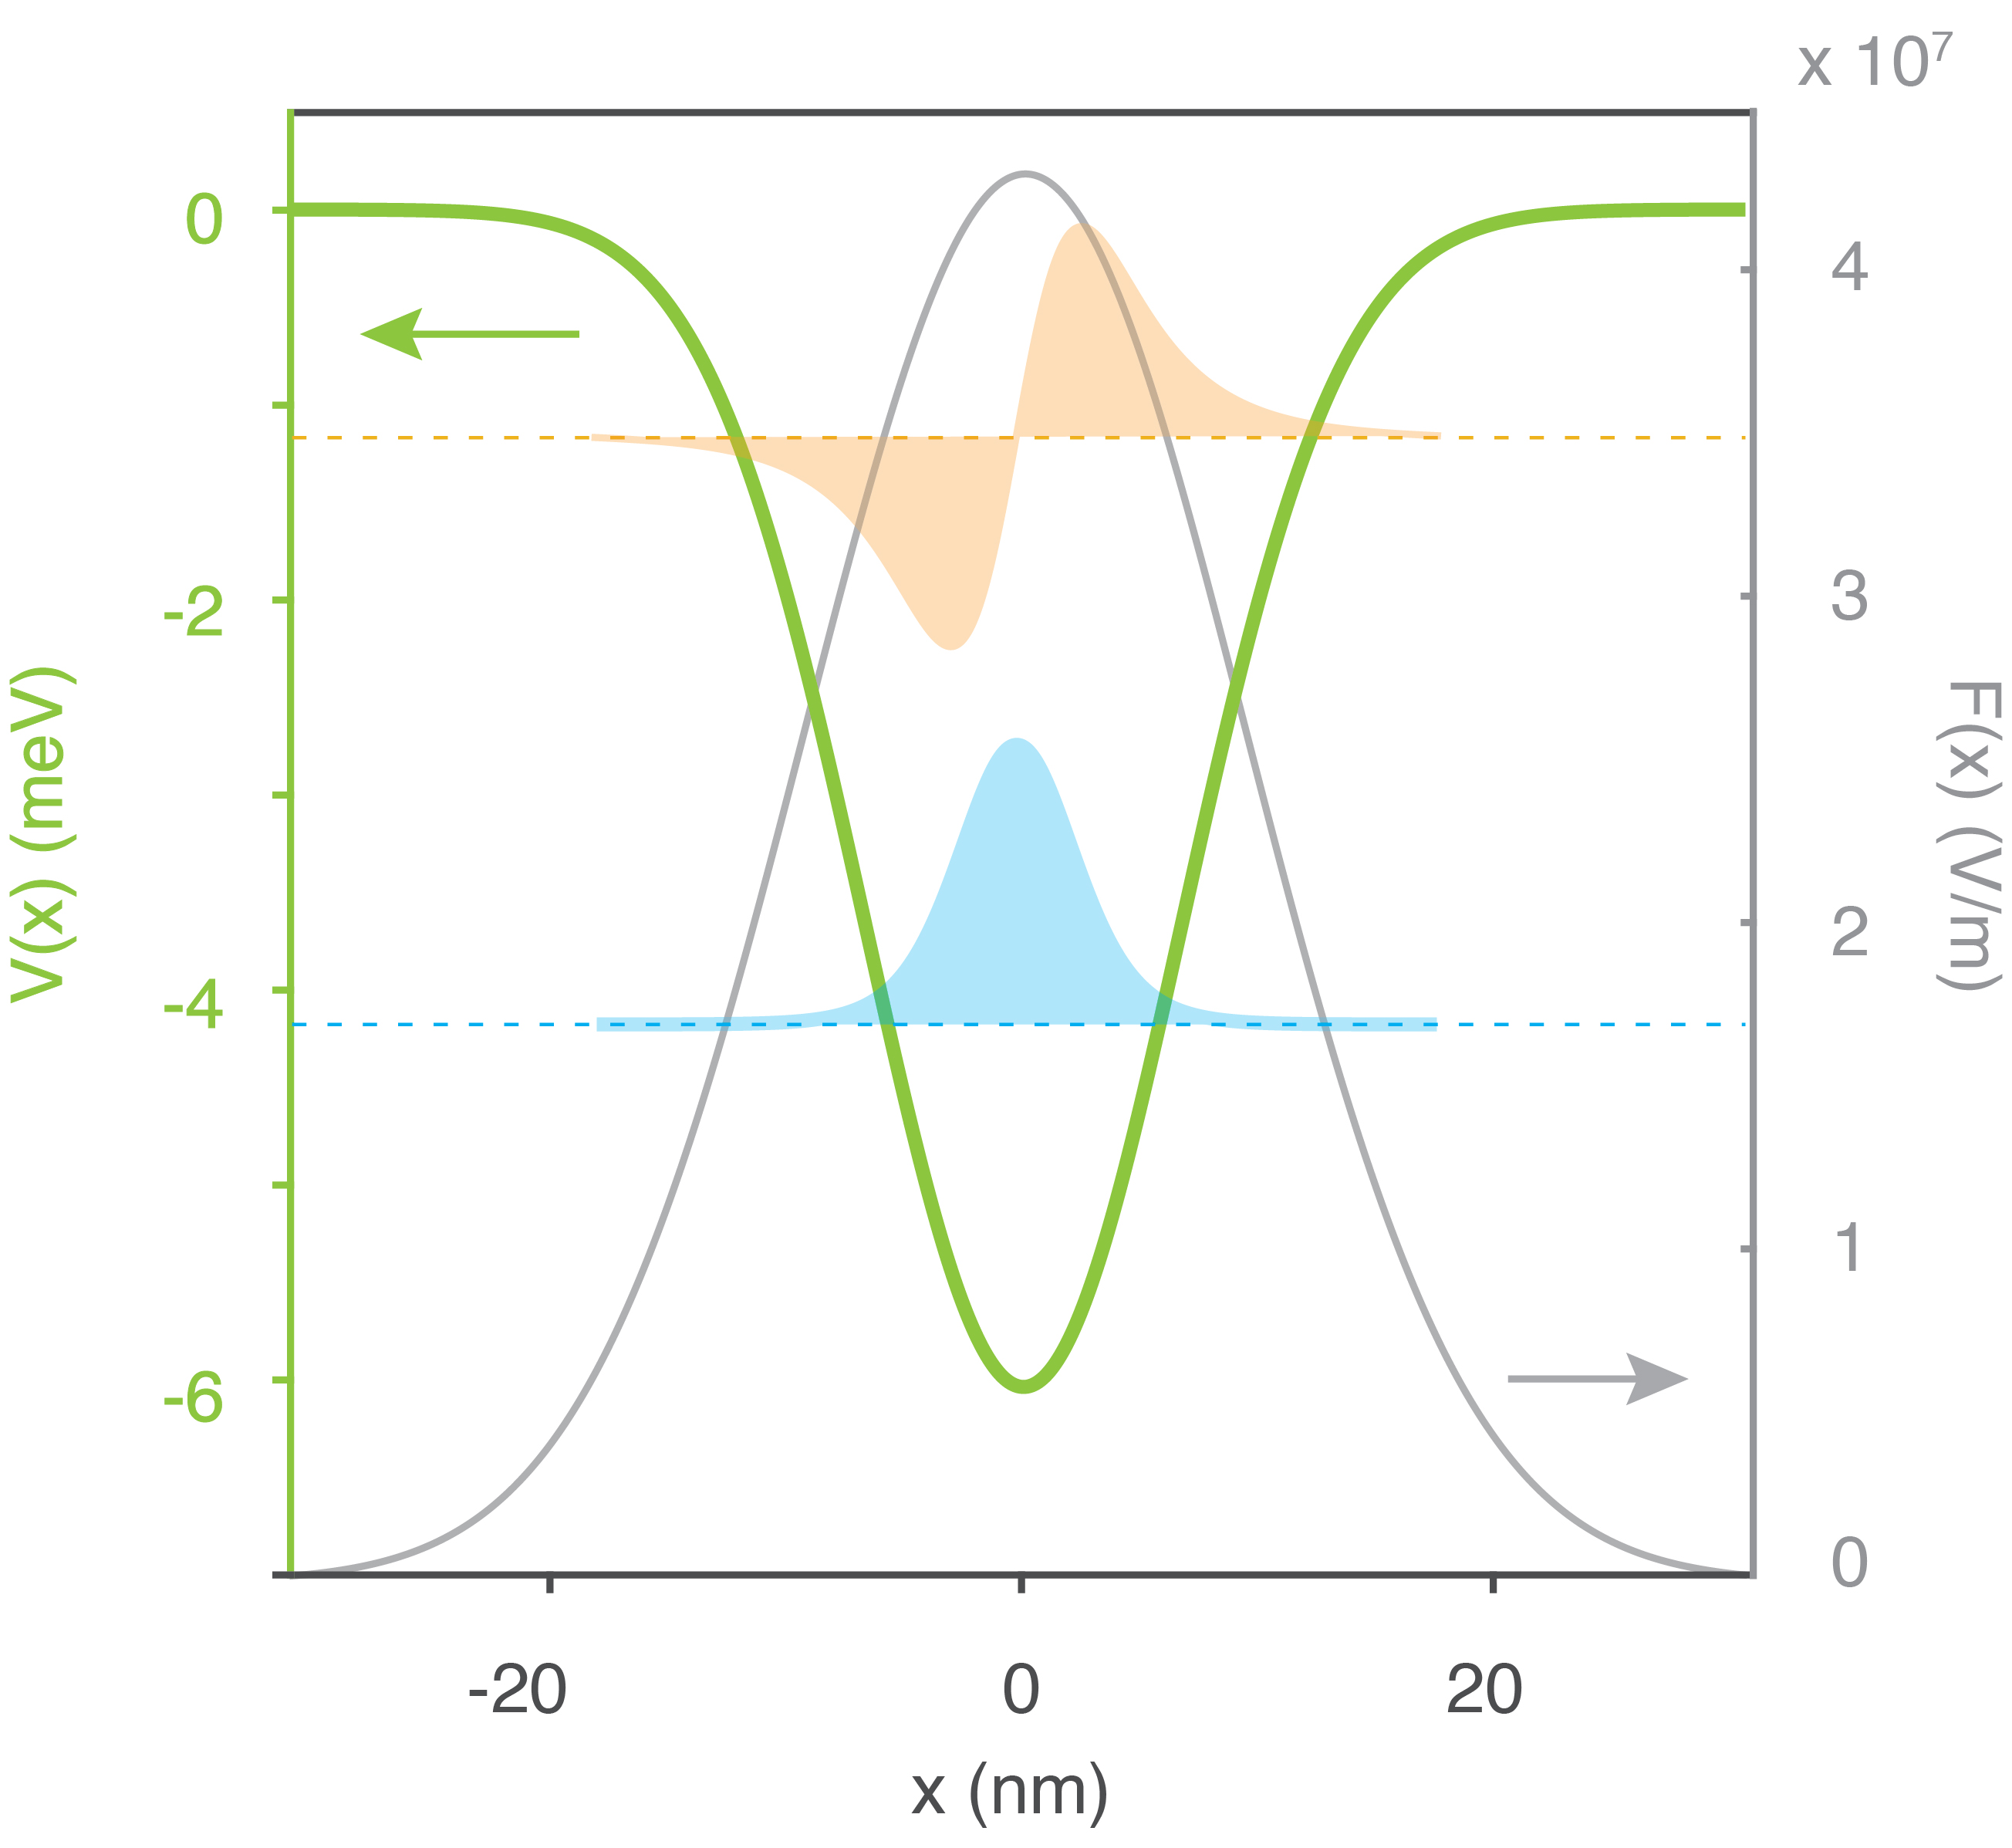
\includegraphics[width=0.5\textwidth]{Figures/C4/figure-S8.jpg} % 
\end{center}
\caption[potential well calculation] {Calculated in-plane electric field \textit{F}(x) (in grey line), confining potential \textit{V}(x) (in green line), and the exciton eigenstates at the 1 $~\mu$m domain region.}
\label{fig.s8}
\end{figure}
\end{quote}
\renewcommand{\baselinestretch}{2}
\small\normalsize
%////////////////Figure End////////////////

\section{Conclusions}

We exploit the recently discovered moiré ferroelectricity in twisted hexagonal boron nitride (hBN) to imprint nanoscale potentials on excitons in 2D semiconductors. 
The strong in-plane electric fields localized at the moiré domain boundaries (DBs) modify the optical reflectance of  MoSe$_2$, indicating that excitons can be confined within a strips as narrow as $\sim$ 10 nanometers. 
The quasi-one-dimensional nature of this confinement is further evidenced by the linear polarization of their optical reflectance. 
In addition, the same fields impose even stronger confinement on Rydberg excitons due to their larger polarizability.

The demonstrated quantum confinement of intralayer excitons at moiré domain walls opens exciting new avenues for controlling excitons at the nanoscale. 
Such a strong in-plane electric field is expected to occur in many types of twisted hetero-structures with broken inversion symmetry \cite{Sung2020-ru}, which can be readily integrated with all sorts of 2D semiconductors to engineer their electronic and excitonic properties\cite{Akamatsu2021-uo,Hu2023-px,He2024-se,Zhang2024-zi}. 
The ferroelectric response observed in many of such twisted structures could enable dynamic electrical control of 1D exciton chains\cite{Kim2025-jv,Vizner-Stern2021-gx,Yasuda2024-qd}. 
The excitonic potential imposed by such an electrostatic lattice — ranging from a few to tens of millielectronvolts — can be tuned to be comparable to the exciton interaction strength\cite{Gu2024-en,Datta2022-po,Tagarelli2023-an,Gu2021-cu,Wang2018-pz}. 
This opens intriguing opportunities for investigating how the interplay between confinement and correlation can give rise to emergent properties in strongly interacting many-body quantum systems, such as quantum optical nonlinearity. 
By employing Rydberg excitons, one can access a compelling regime in which the confinement length scale is comparable to the exciton blockade radius, analogous to one-dimensional Rydberg atom chains\cite{Endres2016-zd,Firstenberg2013-to,Roy2017-nd}. 
To access this intriguing regime, new optical methods may be required to investigate how light interacts with the 1D excitonic chains as it propagates along and within the domain walls, such as near-field techniques\cite{Zhang2022-ty,Crottini2001-lg}.